%Dokumentklasse
\documentclass[a4paper,11pt]{scrreprt}
\usepackage[left= 3.5cm,right = 3cm, bottom = 3.5 cm, top = 3 cm]{geometry}
\usepackage[onehalfspacing]{setspace}
% ============= Packages =============


%==========Drak Mode=================

\usepackage{xcolor}
\definecolor{textStd}{rgb}{0.5, 0.55, 0.6}
\definecolor{bgStd}{rgb}{0.09804, 0.1059, 0.1216}

\definecolor{citeStd}{rgb}{0.7, 0.52, 0.15}

% \definecolor{citeStd}{rgb}{0.7, 0.72, 0.75}
% \definecolor{urlStd}{rgb}{0.3, 0.32, 0.95}
\definecolor{urlStd}{rgb}{0.7, 0.52, 0.15}

\definecolor{COMP}{rgb}{0.402, 0.402, 0.402}

\pagecolor{bgStd}
\color{textStd}

%===================================


%==========Light Mode=================

% \usepackage{xcolor}
% \definecolor{textStd}{rgb}{0., 0., 0.}
% \definecolor{bgStd}{rgb}{1, 1, 1}
% \definecolor{citeStd}{rgb}{0.1, 0.1, 0.75}
% \definecolor{urlStd}{rgb}{0.1, 0.1, 0.95}
% \definecolor{COMP}{rgb}{0.102, 0.102, 0.102}

% \pagecolor{bgStd}
% \color{textStd}

%===================================



% Dokumentinformationen
\usepackage[
	pdftitle={EPRO TD Freifach},
	pdfsubject={},
	pdfauthor={Patrik Lechner},
	pdfkeywords={}
	pdftex=true,
	colorlinks=true,
 	breaklinks=true,
	citecolor=citeStd,
	linkcolor=citeStd,
	menucolor=citeStd,
	urlcolor=citeStd
]{hyperref}

\hypersetup{
    bookmarks=true,         % show bookmarks bar?
    unicode=false,          % non-Latin characters in Acrobat’s bookmarks
    pdftoolbar=true,        % show Acrobat’s toolbar?
    pdfmenubar=true,        % show Acrobat’s menu?
    pdffitwindow=false,     % window fit to page when opened
    pdfstartview={FitH},    % fits the width of the page to the window
    pdftitle={My title},    % title
    pdfauthor={Author},     % author
    pdfsubject={Subject},   % subject of the document
    pdfcreator={Creator},   % creator of the document
    pdfproducer={Producer}, % producer of the document
    pdfkeywords={keyword1} {key2} {key3}, % list of keywords
    pdfnewwindow=true,      % links in new window
    colorlinks=true,       % false: boxed links; true: colored links
    linkcolor=citeStd,          % color of internal links (change box color with linkbordercolor)
    citecolor=citeStd,        % color of links to bibliography
    filecolor=citeStd,      % color of file links
    urlcolor=urlStd           % color of external links
}

% Standard Packages
\usepackage[utf8]{inputenc}

% deutsch
% \usepackage[ngerman]{babel}
% \usepackage[ngerman, num]{isodate}

% english
\usepackage[english]{babel}

\usepackage[T1]{fontenc}
\usepackage{graphicx}
\usepackage{graphicx, subfigure}
%setze pfad fuer Bilder
% \graphicspath{{img/}}
\usepackage{fancyhdr}
\usepackage{lmodern}
\usepackage{color}
\usepackage{transparent}

% framed, let's us create framed paragraphs.
\usepackage{framed}

% Citation style
\usepackage[comma,authoryear]{natbib}
%\usepackage{natbib}

% zusätzliche Schriftzeichen der American Mathematical Society
\usepackage{amsfonts}
\usepackage{mathtools}


% BlockDiagram Drawing Package
% ---tikz
\usepackage{tikz}
\usetikzlibrary{positioning}
\usepackage{pgfplots}
\pgfplotsset{compat=1.10}
\usepackage{textcomp}

\usetikzlibrary{mindmap,trees, backgrounds}


%Package for using the [H] option on graphics to force them into place
\usepackage{float}


%iPython packages:
\usepackage{graphicx} % Used to insert images
\usepackage{adjustbox} % Used to constrain images to a maximum size
\usepackage{color} % Allow colors to be defined
\usepackage{enumerate} % Needed for markdown enumerations to work
\usepackage{geometry} % Used to adjust the document margins
\usepackage{amsmath} % Equations
\usepackage{amssymb} % Equations
\usepackage[mathletters]{ucs} % Extended unicode (utf-8) support
% \usepackage[utf8x]{inputenc} % Allow utf-8 characters in the tex document
\usepackage{fancyvrb} % verbatim replacement that allows latex
\usepackage{grffile} % extends the file name processing of package graphics
                         % to support a larger range
    % The hyperref package gives us a pdf with properly built
    % internal navigation ('pdf bookmarks' for the table of contents,
    % internal cross-reference links, web links for URLs, etc.)
\usepackage{hyperref}
\usepackage{longtable} % longtable support required by pandoc >1.10


% embedding of audio/video files etc.
% \usepackage{attachfile}
% \usepackage{movie15}
% \usepackage{media9}
% \usepackage{menukeys}





% =============== BlockDiagram Drawing Config
\usetikzlibrary{shapes,arrows}


% Definition of blocks:
\tikzset{%
  block/.style    = {draw, thick, rectangle, minimum height = 3em,
    minimum width = 3em},
  sum/.style      = {draw, circle, node distance = 2cm}, % Adder
  input/.style    = {coordinate}, % Input
  output/.style   = {coordinate}, % Output
  mult/.style	  = {draw, isosceles triangle, minimum height=1cm, minimum width =1cm}
}
%mult/.style	  = {isosceles triangle, sharp corners, anchor=center, xshift=-4mm, minimum height=1.5cm, minimum width =0.05cm}
%isosceles triangle, fill=gray!25, minimum width=1.5cm

% Defining string as labels of certain blocks.
\newcommand{\suma}{\Large$+$}
\newcommand{\inte}{$\displaystyle \int$}
\newcommand{\derv}{\huge$\frac{d}{dt}$}
\newcommand{\conv}{\huge$\ast$}

% ============Shortcut/Keystroke drawing===================

\usetikzlibrary{shadows}

\newcommand*\keystroke[1]{%
  \tikz[baseline=(key.base)]
    \node[%
      draw,
      fill=bgStd,
      drop shadow={shadow xshift=0.25ex,shadow yshift=-0.25ex,fill=textStd,opacity=0.75},
      rectangle,
      rounded corners=2pt,
      inner sep=1pt,
      line width=0.5pt,
      font=\scriptsize\sffamily
    ](key) {#1\strut}
  ;
}


% ============================================

% -- Settings für Code abbildungen
\usepackage{listings}

\definecolor{dkgreen}{rgb}{0,0.6,0}
\definecolor{gray}{rgb}{0.5,0.5,0.5}
\definecolor{mauve}{rgb}{0.58,0,0.82}

\lstset{frame=tb,
  language=Python,
  aboveskip=3mm,
  belowskip=3mm,
  showstringspaces=false,
  columns=flexible,
  basicstyle={\small\ttfamily},
  numbers=none,
  numberstyle=\tiny\color{gray},
  keywordstyle=\color{blue},
  commentstyle=\color{dkgreen},
  stringstyle=\color{mauve},
  breaklines=true,
  breakatwhitespace=true
  tabsize=3
}




% Setze arial font
% \renewcommand*{\familydefault}{\sfdefault}

% FH-grünBlau
\definecolor{FH}{rgb}{0.10, 0.57, 0.68}

% touchDesigner specific

\definecolor{TOP}{rgb}{0.349, 0.310, 0.482}
\definecolor{CHOP}{rgb}{0.369, 0.518, 0.275}
\definecolor{SOP}{rgb}{0.271, 0.451, 0.624}
\definecolor{MAT}{rgb}{0.569, 0.533, 0.271}
\definecolor{DAT}{rgb}{0.529, 0.341, 0.475}


\newcommand{\link}[2]{\href{#1}{#2}\footnote{#1}}


\newcommand{\refTOP}[1]{\href{http://derivative.ca/wiki099/index.php?title=#1\_TOP}{#1 \TOP}\footnote{http://derivative.ca/wiki099/index.php?title=#1\_TOP}}

% nicht einrücken nach Absatz
\setlength{\parindent}{0pt}


% ============= Kopf- und Fußzeile =============
\pagestyle{fancy}
%
\lhead{}
\chead{}
\rhead{\slshape \leftmark}
%%
\lfoot{}
\cfoot{}
\rfoot{\thepage}
%%
\renewcommand{\headrulewidth}{0.4pt}
\renewcommand{\footrulewidth}{0pt}

% ============= Remove first Page======

\usepackage{atbegshi}% http://ctan.org/pkg/atbegshi
\AtBeginDocument{\AtBeginShipoutNext{\AtBeginShipoutDiscard}}

%======================================


% ============= Package Einstellungen & Sonstiges =============

%Besondere Trennungen
\hyphenation{De-zi-mal-tren-nung St-rei-fen-licht-scan-nern}

%römische Aufzählungen mit \RM{Zahl}
\newcommand{\RM}[1]{\MakeUppercase{\romannumeral #1}}

% ============= TouchDesigner Specific =============
\usepackage{xspace} %makes sure the spacing is alright when using the
% function below.

% these are definitions that seem to need to be copied into each chapter file...
% they are only here so there's a central reference that should be correct.

\def\boldcommandlist{\@elt OP,\@elt OPs,}
\def\@elt#1,{%
 \expandafter\def\csname#1\endcsname{\textbf{#1}\xspace}
}
\boldcommandlist

\def\topColorList{\@elt TOP,\@elt TOPs,}
\def\@elt#1,{%
 \expandafter\def\csname#1\endcsname{\textcolor{TOP}{\textbf{#1}}\xspace}
}
\topColorList

\def\chopColorList{\@elt CHOP,\@elt CHOPs,}
\def\@elt#1,{%
 \expandafter\def\csname#1\endcsname{\textcolor{CHOP}{\textbf{#1}}\xspace}
}
\chopColorList

\def\sopColorList{\@elt SOP,\@elt SOPs,}
\def\@elt#1,{%
 \expandafter\def\csname#1\endcsname{\textcolor{SOP}{\textbf{#1}}\xspace}
}
\sopColorList

\def\datColorList{\@elt DAT,\@elt DATs,}
\def\@elt#1,{%
 \expandafter\def\csname#1\endcsname{\textcolor{DAT}{\textbf{#1}}\xspace}
}
\datColorList

\def\matColorList{\@elt MAT,\@elt MATs,}
\def\@elt#1,{%
 \expandafter\def\csname#1\endcsname{\textcolor{MAT}{\textbf{#1}}\xspace}
}
\matColorList


\def\compColorList{\@elt COMP,\@elt COMPs,}
\def\@elt#1,{%
 \expandafter\def\csname#1\endcsname{\textcolor{COMP}{\textbf{#1}}\xspace}
}
\compColorList


\def\redcommandlist{\@elt missingImage,}
\def\@elt#1,{%
 \expandafter\def\csname#1\endcsname{\textcolor{red}{\textbf{#1}}\xspace}
}
\redcommandlist

% =====indizierung
\usepackage{makeidx}
\makeindex

% ===================================================


% ============= Dokumentbeginn =============

\begin{document}

% \include{01_titel}
%!TEX root = main.tex
\color{textStd}

\pagestyle{empty}
\begin{center}
\begin{tabular}{p{\textwidth}}

% \begin{center}
% 
\includegraphics[scale=0.7]{./img/FHlogo.jpg}
% \end{center}

\\

\begin{center}
\Huge{{\color{FH}{\fontsize{24}{48} \selectfont TouchDesigner Course\\}}}
\end{center}

\\

\\

\begin{center}
% Medientechnik\\
% University of Applied Sciences St.Pölten
\end{center}


\begin{center}
\large{\textbf{Patrik Lechner}} \\

\end{center}

\\

\\

\begin{center}
\large{Vienna, \today}
\end{center}



% \begin{center}
% \large{\LaTeX}
% \end{center}

\end{tabular}
\end{center}
%!TEX root = main.tex
\color{textStd}

\pagestyle{empty}
\begin{center}
\begin{tabular}{p{\textwidth}}

% \begin{center}
% 
\includegraphics[scale=0.7]{./img/FHlogo.jpg}
% \end{center}

\\

\begin{center}
\Huge{{\color{FH}{\fontsize{24}{48} \selectfont TouchDesigner Course\\}}}
\end{center}

\\

\\

\begin{center}
% Medientechnik\\
% University of Applied Sciences St.Pölten
\end{center}


\begin{center}
\large{\textbf{Patrik Lechner}} \\

\end{center}

\\

\\

\begin{center}
\large{Vienna, \today}
\end{center}



% \begin{center}
% \large{\LaTeX}
% \end{center}

\end{tabular}
\end{center}
% \part im Inhaltsverzeichnis nicht nummerieren
\makeatletter
\let\partbackup\l@part
\renewcommand*\l@part[2]{\partbackup{#1}{}}

%Seitennummerierung neu beginnen, Zahlen [arabic], röm.Zahlen [roman,Roman], Buchstaben [alph,Alph]
\pagenumbering{Roman}

\newpage
%
%!TEX root = main.tex
%=================TD functions==================

\def\boldcommandlist{\@elt OP,\@elt OPs,}
\def\@elt#1,{%
 \expandafter\def\csname#1\endcsname{\textbf{#1}\xspace}
}
\boldcommandlist

\def\topColorList{\@elt TOP,\@elt TOPs,}
\def\@elt#1,{%
 \expandafter\def\csname#1\endcsname{\textcolor{TOP}{\textbf{#1}}\xspace}
}
\topColorList

\def\chopColorList{\@elt CHOP,\@elt CHOPs,}
\def\@elt#1,{%
 \expandafter\def\csname#1\endcsname{\textcolor{CHOP}{\textbf{#1}}\xspace}
}
\chopColorList

\def\sopColorList{\@elt SOP,\@elt SOPs,}
\def\@elt#1,{%
 \expandafter\def\csname#1\endcsname{\textcolor{SOP}{\textbf{#1}}\xspace}
}
\sopColorList

\def\datColorList{\@elt DAT,\@elt DATs,}
\def\@elt#1,{%
 \expandafter\def\csname#1\endcsname{\textcolor{DAT}{\textbf{#1}}\xspace}
}
\datColorList

\def\matColorList{\@elt MAT,\@elt MATs,}
\def\@elt#1,{%
 \expandafter\def\csname#1\endcsname{\textcolor{MAT}{\textbf{#1}}\xspace}
}
\matColorList


\def\compColorList{\@elt COMP,\@elt COMPs,}
\def\@elt#1,{%
 \expandafter\def\csname#1\endcsname{\textcolor{COMP}{\textbf{#1}}\xspace}
}
\compColorList


%===============================================


% \def\boldcommandlist{\@elt FS,\@elt OFS,\@elt RS,\@elt ORS,\@elt NR,\@elt NF,\@elt FNR,}
% \def\@elt#1,{%
%  \expandafter\def\csname#1\endcsname{\textbf{#1}\xspace}
% }
% \boldcommandlist
\color{textStd}

\addsec{Introduction/Notes}
\label{Notes}


\section{Notes} % (fold)
\label{notes}

Video playback

\subsection{Project Ideas}
\label{sub:ideen}
\subsubsection{Simple}
\begin{itemize}
	\item Hipster filter
	\item Audio Reactive Noise Ball
	\item Toon Shader
	\item Replicator Experiments
	\item Oscilloscope/Spectroscope
	\item leap motion
\end{itemize}

\subsubsection{Intermediate}
\begin{itemize}
	\item \glqq{}Auto-Cutter\grqq{}
	\item Particle stuff
	\item DMX
	\item big-data viz
\end{itemize}

\subsubsection{Long Term}
\begin{itemize}
	\item Mapping
	\item Music Video
	\item Aiko Aiko
	\item Procedural Modelling (Bicycle, House, ...)
	\item (3d) Multi-Touch Interface
	\item vj-app
	\item (Light) Show Simulation
	\item Color Grading Software
	\item video Analysis


\end{itemize}

\section{Course Structure} % (fold)

% \def\boldcommandlist{\@elt OP,\@elt OFS,\@elt RS,\@elt ORS,\@elt NR,\@elt NF,\@elt FNR,}
% \def\@elt#1,{%
%  \expandafter\def\csname#1\endcsname{\textbf{#1}\xspace}
% }
% \boldcommandlist


\subsection{Lecture 1 introduction and 2D-processing} % (fold)
\label{sub:lecture_1}
\begin{itemize}
	\item students show what they want to do in form of images in a toe file.
	\item showing off what TD can do, what I did so far.
	% \item history of TD (Houdini) and comparison to other similar software
	% \item possibly quick intro to latex/github for collaborative work on this
	\item Intro to TD
		\begin{itemize}
		\item getting help
		\item the GUI (quick overview)
		\item the \OPs
		\item in Depth: \TOPs and \CHOPs
		\item first guided projects
		% \item overview over useful \DATs
		% \item GUI more in depth (or rather do this along the way?)
		\item first python expressions (just something like \verb|absTime.frame/100|)
		\item a very quick look at GUIs
		\item output window handling and MovieFileOut \TOP. Possibly but rather not: off-line rendering.
		\end{itemize}
	% \item semester project groups and topics choice
\end{itemize}

\subsection{Lecture 2, Rendering Setup and Procedural Modeling}
\label{sub:lecture_2}
\begin{itemize}
	\item encapsulating Work, \COMPs
	\item converting between OP families, and why
	\item GUIs again
	\item Select \OPs
	% \item audio: filter \CHOPs, spectrum \CHOP, analysis \CHOP
	\item Render Setup
	\item some fun SOPs: copy, group, noise, facet, particle, magnet, force, twist, lattice
	\item feedback \TOP
	\item lights, light projection, shadows
	\item off-line rendering
\end{itemize}

\subsection{Lecture 3, Replication and Instancing, compositing and more project structure}
\label{sub:lecture_3}
\begin{itemize}
	\item instancing
	\item particle rendering
	\item replicator \COMP
	\item Clones
	\item render pass \TOP
\end{itemize}

\subsection{Lecture 4}
\label{sub:lecture_4}
\begin{itemize}
	\item Scripting
	\item Projection Mapping
	\item DATA/API visualization
\end{itemize}


\subsection{Lecture 5}
\label{sub:lecture_5}
% \itemize
Working on the final Project

\subsection{Lecture 6, project presentation}
\label{sub:lecture_6}




\newpage


\newpage
\pagestyle{fancy}
%Inhaltsverzeichnis
\tableofcontents

\newpage
%Seitennummerierung neu beginnen, Zahlen [arabic], röm.Zahlen [roman,Roman], Buchstaben [alph,Alph]
\pagenumbering{arabic}

% pagestyle für gesamtes Dokument aktivieren
\pagestyle{fancy}


\newpage

% \@addtoreset{chapter}{part}
%!TEX root = main.tex


% \begin{center}
% \begin{figure}[h!]
% \tikzset{concept/.append style={fill={none}}}
% \begin{tikzpicture}
%   \path[mindmap,concept color=black,text=black]
%     node[concept] {Inroduction}
%     [clockwise from=0]
%     child[concept color=CHOP] {
%       node[concept] {CHOPs}
%       % }
%       [clockwise from=90]
%       child { node[concept] {Exporting} }
%       % child { node[concept color=green] {CHOPs} }
%       % child { node[concept] {TOPs} }
%       % child { node[concept] {pro\-gramming languages} }
%       % child { node[concept] {software engineer\-ing} }
%     }
%     child[concept color=TOP] {
%       node[concept] (fm) {TOPs}
%       [clockwise from=-30]
%     }
%     child[concept color=blue] { node[concept] (pm){GUI}
%         [clockwise from=180] child[concept]{node[concept] {Navigation and COMPS}}
%         }
%     child[concept color=red] { node[concept] (si) {Student's interests} }
%     child[concept color=orange] { node[concept] (op) {Output}
%         [clockwise from=180] child[concept]{node[concept]{Realtime
%         }}
%         child[concept]{node[concept]{Movie Out
%         }}
%     };


% % \begin{pgfonlayer}{background}
% %     \draw [circle connection bar]
% %       (fm) edge (sd)
% %       (fm) edge (pm);
% %   \end{pgfonlayer}

% \end{tikzpicture}
% \caption{Lecture 1}
% \end{figure}
% \end{center}

% Lorem ipsum dolor sit amet, consectetur adipisicing elit, sed do eiusmod
% tempor incididunt ut labore et dolore magna aliqua. Ut enim ad minim veniam,
% quis nostrud exercitation ullamco laboris nisi ut aliquip ex ea commodo
% consequat. Duis aute irure dolor in reprehenderit in voluptate velit esse
% cillum dolore eu fugiat nulla pariatur. Excepteur sint occaecat cupidatat non
% proident, sunt in culpa qui officia deserunt mollit anim id est laborum.

% \begin{center}
% \begin{figure}[h!]
% % \tikzset{concept/.append style={fill={none}}}
% \begin{tikzpicture}
%   \path[mindmap,concept color=black,text=black]
%   node[concept] {Inroduction};
% \end{center}
% \end{figure}
% \end{tikzpicture}


% \begin{center}
% \begin{figure}[h!]
% \tikzset{concept/.append style={fill={none}}}
% \begin{tikzpicture}
%   % \path[mindmap]
%     node[concept] {Inroduction};
%     [clockwise from=0]
%     child[concept color=SOP] {
%       node[concept] {SOPs}
%       % }
%       [clockwise from=90]
%       child { node[concept] {Exporting} }
%       % child { node[concept color=green] {CHOPs} }
%       % child { node[concept] {TOPs} }
%       % child { node[concept] {pro\-gramming languages} }
%       % child { node[concept] {software engineer\-ing} }
%     }
%     child[concept color=TOP] {
%       node[concept] (tops) {TOPs}
%       [clockwise from=-30]
%     }
%     child[concept color=blue] { node[concept] (gui){GUI}
%         [clockwise from=180] child[concept]{node[concept] {Navigation and COMPS}}
%         }
%     child[concept color=red] { node[concept] (interr) {Student's interests} }
%     child[concept color=orange] { node[concept] (outp) {Output}
%         [clockwise from=180] child[concept]{node[concept]{Realtime
%         }}
%         child[concept]{node[concept]{Movie Out
%         }}
%     };
% \end{tikzpicture}
% \caption{Lecture 2}
% \end{figure}
% \end{center}


%!TEX root = main.tex
%=================TD functions==================
\def\boldcommandlist{\@elt OP,\@elt OPs,}
\def\@elt#1,{%
 \expandafter\def\csname#1\endcsname{\textbf{#1}\xspace}
}
\boldcommandlist

\def\topColorList{\@elt TOP,\@elt TOPs,}
\def\@elt#1,{%
 \expandafter\def\csname#1\endcsname{\textcolor{TOP}{\textbf{#1}}\xspace}
}
\topColorList

\def\chopColorList{\@elt CHOP,\@elt CHOPs,}
\def\@elt#1,{%
 \expandafter\def\csname#1\endcsname{\textcolor{CHOP}{\textbf{#1}}\xspace}
}
\chopColorList

\def\sopColorList{\@elt SOP,\@elt SOPs,}
\def\@elt#1,{%
 \expandafter\def\csname#1\endcsname{\textcolor{SOP}{\textbf{#1}}\xspace}
}
\sopColorList

\def\datColorList{\@elt DAT,\@elt DATs,}
\def\@elt#1,{%
 \expandafter\def\csname#1\endcsname{\textcolor{DAT}{\textbf{#1}}\xspace}
}
\datColorList

\def\matColorList{\@elt MAT,\@elt MATs,}
\def\@elt#1,{%
 \expandafter\def\csname#1\endcsname{\textcolor{MAT}{\textbf{#1}}\xspace}
}
\matColorList


\def\compColorList{\@elt COMP,\@elt COMPs,}
\def\@elt#1,{%
 \expandafter\def\csname#1\endcsname{\textcolor{COMP}{\textbf{#1}}\xspace}
}
\compColorList

\def\redcommandlist{\@elt missingImage,}
\def\@elt#1,{%
 \expandafter\def\csname#1\endcsname{\textcolor{red}{\textbf{#1}}\xspace}
}
\redcommandlist




%===============================================

\chapter{Lecture 1, Introduction and 2D-Processing}
\label{chap:Introduction}
\section{Notes}
\color{textStd}

\begin{center}
\begin{figure}[h!]
\tikzset{concept/.append style={fill={none}}}
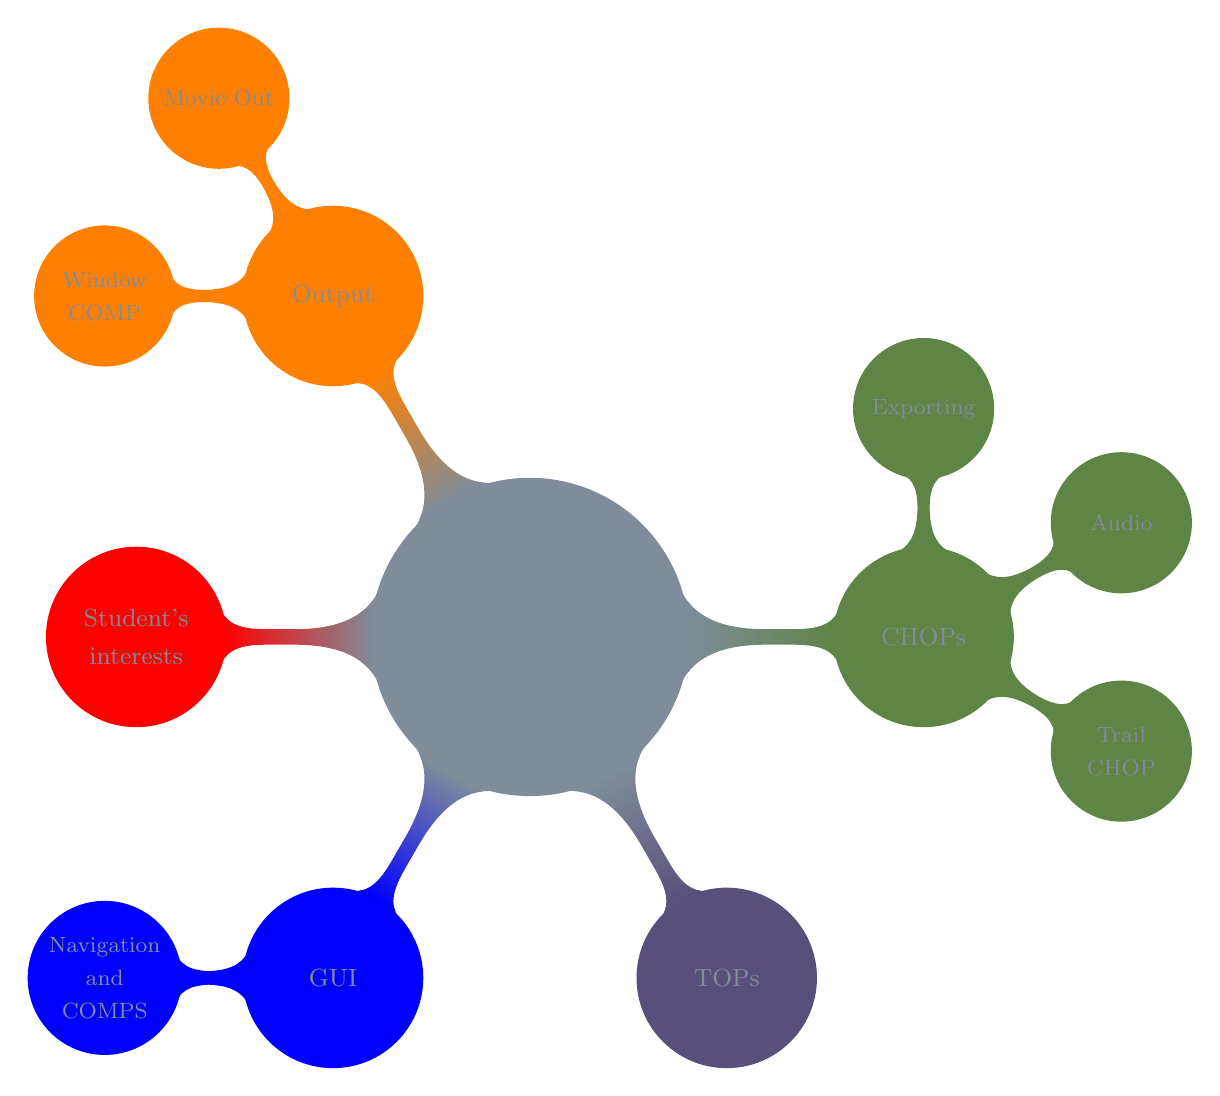
\begin{tikzpicture}
  \path[mindmap,concept color=textStd,text=textStd]
    node[concept] {Introduction}
    [clockwise from=0]
    child[concept color=CHOP] {
      node[concept] {CHOPs}
      % }
      [clockwise from=90]
      child { node[concept] {Exporting} }
      child { node[concept] {Audio} }
      child { node[concept] {Trail CHOP} }
      % child { node[concept] {TOPs} }
      % child { node[concept] {pro\-gramming languages} }
      % child { node[concept] {software engineer\-ing} }
    }
    child[concept color=TOP] {
      node[concept] (fm) {TOPs}
      [clockwise from=-30]
    }
    child[concept color=blue] { node[concept] (pm){GUI}
        [clockwise from=180] child[concept]{node[concept] {Navigation and COMPS}}
        }
    child[concept color=red] { node[concept] (si) {Student's interests} }
    child[concept color=orange] { node[concept] (op) {Output}
        [clockwise from=180] child[concept]{node[concept]{Window COMP
        }}
        child[concept]{node[concept]{Movie Out
        }}
    };


% \begin{pgfonlayer}{background}
%     \draw [circle connection bar]
%       (fm) edge (sd)
%       (fm) edge (pm);
%   \end{pgfonlayer}

\end{tikzpicture}
\caption{Lecture Contents}
\end{figure}
\end{center}

% \begin{figure}[H]
% 	\begin{center}
% 		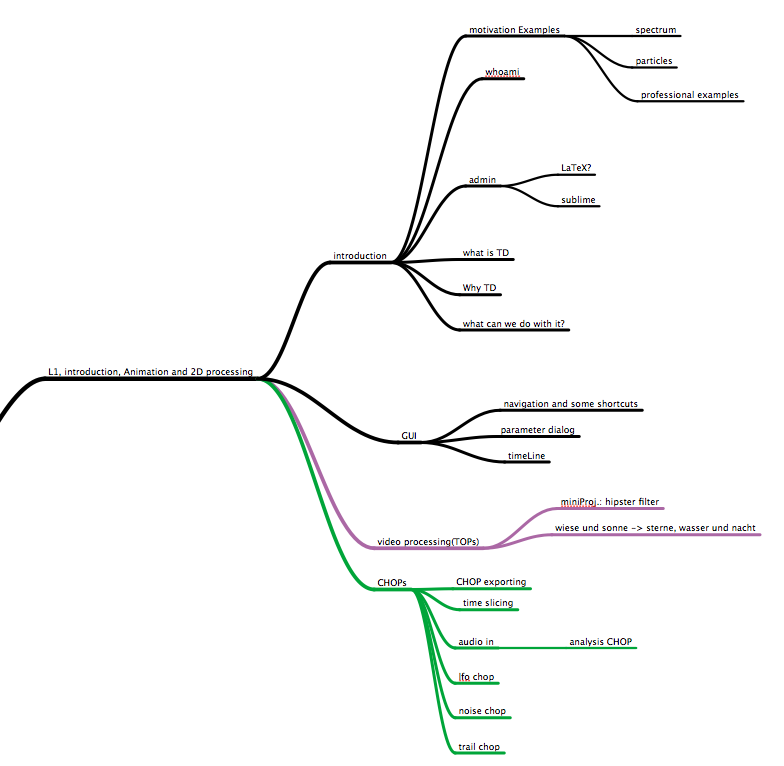
\includegraphics[width = 18cm]{img/lecture1.png}
% 		\caption{overview}
% 		\label{fig:overview}
% 	\end{center}
% \end{figure}

\section{About}

About me:
\link{http://www.vimeo.com/titled}{my vimeo site}
% \href


TouchDesigner is coming from sideFX/Houdini. Now made by the company \textit{derivative} \\

Other products, more or less similar to TD:
\begin{itemize}
	\item vvvv
	\item quarz composer
	\item Max/MSP/Jitter
	\item processing
	\item also game engines(Unity, Unreal, ...)
\end{itemize}

What can we do with TD?
\begin{itemize}
	\item \link{https://www.derivative.ca/Events/2014/Gravity/}{gravity}
	\item \link{https://vimeo.com/55818038}{v squares Mapping Reel}
	\item \link{https://vimeo.com/groups/touchdesigner/videos/71991897}{NiN tour}
\end{itemize}


% projects in this lecture:
% \begin{itemize}
% 	\item hipster filter
% 	\item video playback (mention ffmpeg, hap encoding)
% 	\item sunRise -> water, stars, night
% 	\item fist rendering
% 	\item noise ball
% 	\item off-line rendering
% \end{itemize}
% subsection subsection_name (end)

\section{Getting Help}
\begin{itemize}
	\item Here (in the future hopefully)
	\item The Book \link{http://www.amazon.com/Multimedia-Programming-using-Max-TouchDesigner/dp/1849699712}{Multimedia Programming using Max/MSP and TouchDesigner}
	\item The open source book \link{http://book.nvoid.com/}{introduction to TouchDesigner}
	\item \link{http://www.derivative.ca/wiki088/index.php?title=Main\_Page}{the TD Wiki}
	\item the TouchDesigner OP Snippets. A useful collection of examples for each operator, accessible via TouchDesigner's help menu.
	\item \link{http://www.derivative.ca/Forum/}{The TD Forums}
	\item \link{https://www.facebook.com/groups/touchdesignerhelp/}{the TouchDesigner Help Group on Facebook}
\end{itemize}

\section{The User Interface} % (fold)
\label{sub:the_user_interface}

In figure \ref{fig:ui} we can see the graphical user interface of TD. Two good videos explaining the first steps(like navigating in the UI etc.) are:
\begin{itemize}
	\item \link{https://vimeo.com/10056323}{Part A}
	\item \link{https://vimeo.com/10106354}{Part B}
\end{itemize}

\begin{figure}[H]
	\begin{center}
		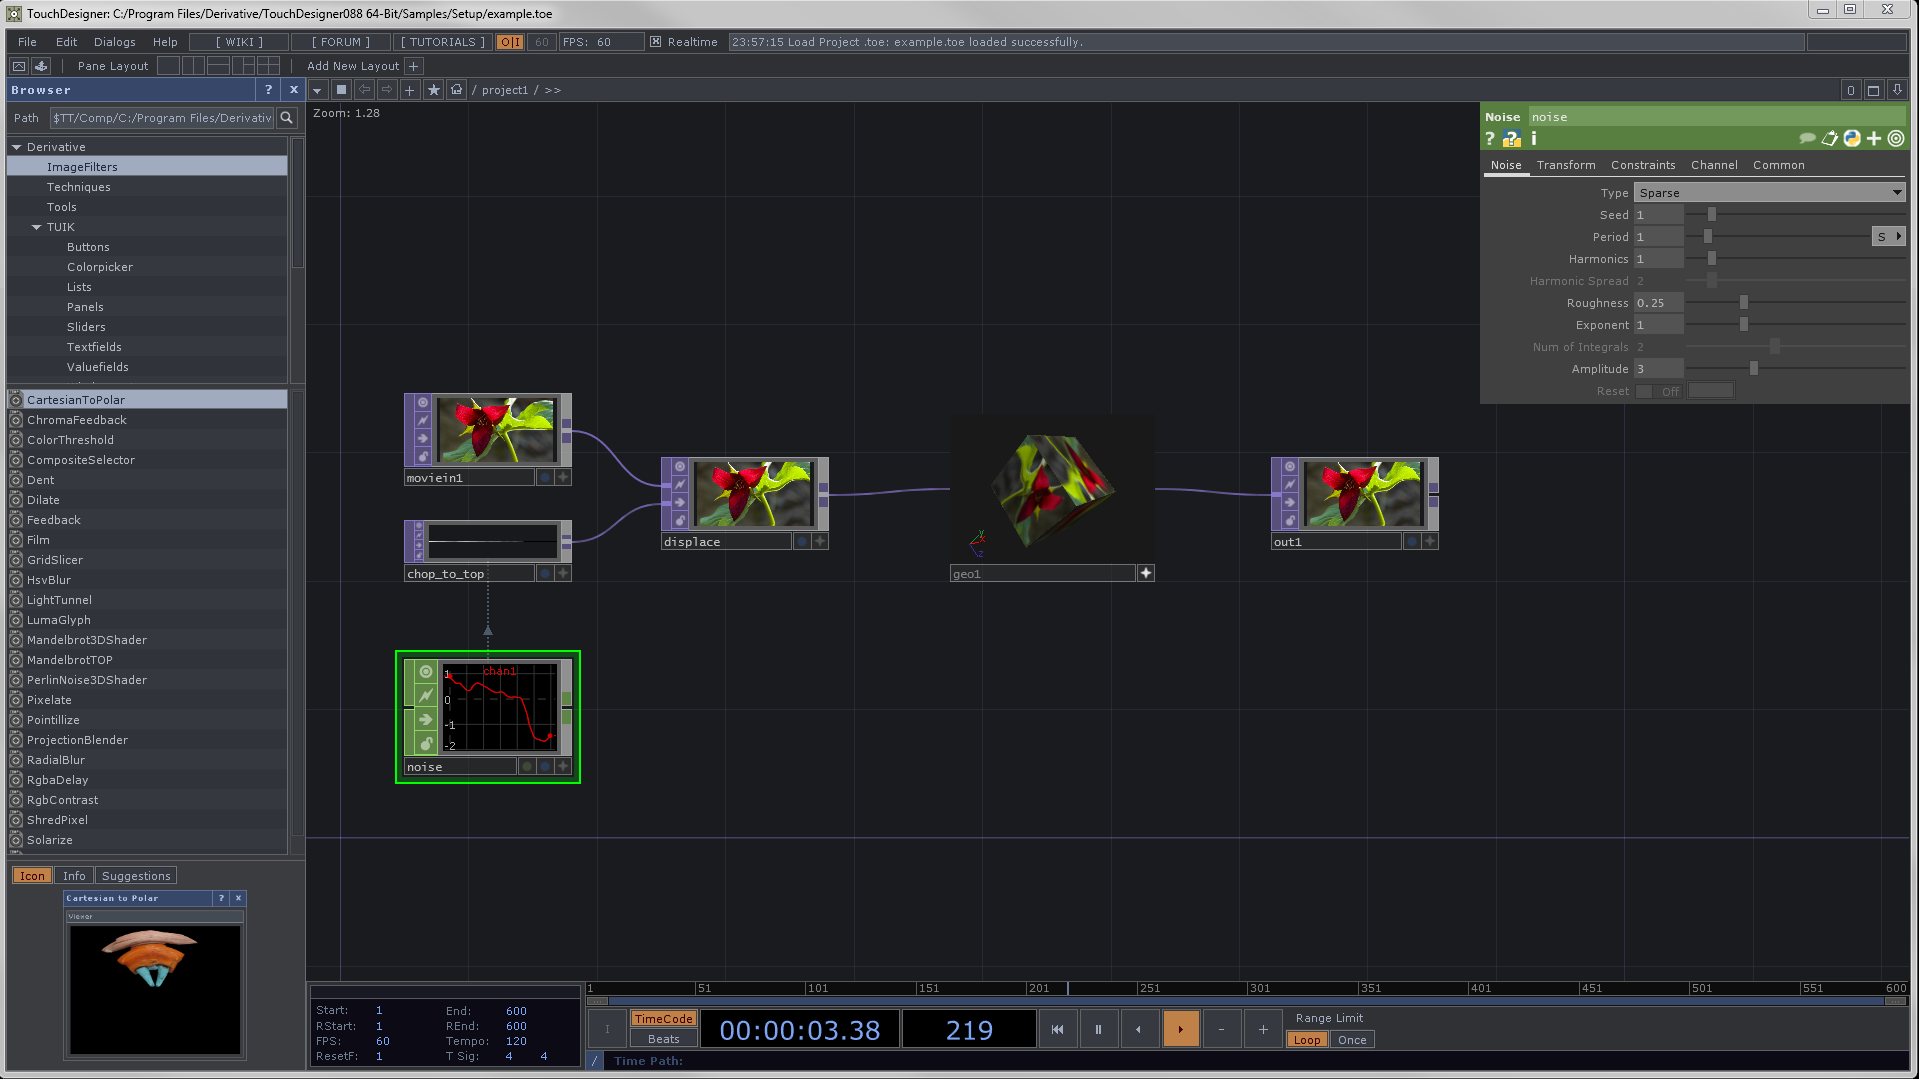
\includegraphics[width = 14cm]{img/gui.png}
		\caption{The User Interface}
		\label{fig:ui}
	\end{center}
\end{figure}

To the left, there is the \textbf{Palette Browser} \index{Palette Browser}, which holds reusable code, \COMPs, made by us or the factory. The big area in the center is called a \textbf{pane} \index{Pane}. Here we can see our \textbf{network}, consisting of operators, or \OPs for short.\\
To the upper right, we have the \textbf{Parameter Dialog}, see also fig. \ref{fig:parDialog},which holds all the options for a currently selected \OP\footnote{In TD we can select multiple \OPs using box selection or the shift key. When we select similar \OPs we can adjust all their values at once in the parameter dialog }.\\

\begin{figure}[H]
	\begin{center}
		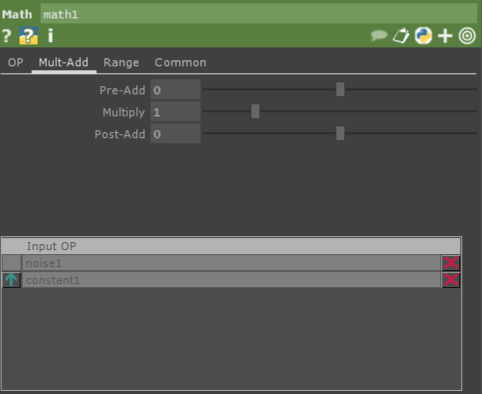
\includegraphics[width = 10cm]{img/parameterDialog.png}
		\caption{the Parameter Dialog}
		\label{fig:parDialog}
	\end{center}
\end{figure}

We can add \OPs by pressing \keystroke{tab} or double clicking in an empty area of the network, to bring up the \textbf{OP Create Dialog}, as depicted in fig. \ref{fig:opCreate}. \\

\begin{figure}[H]
	\begin{center}
		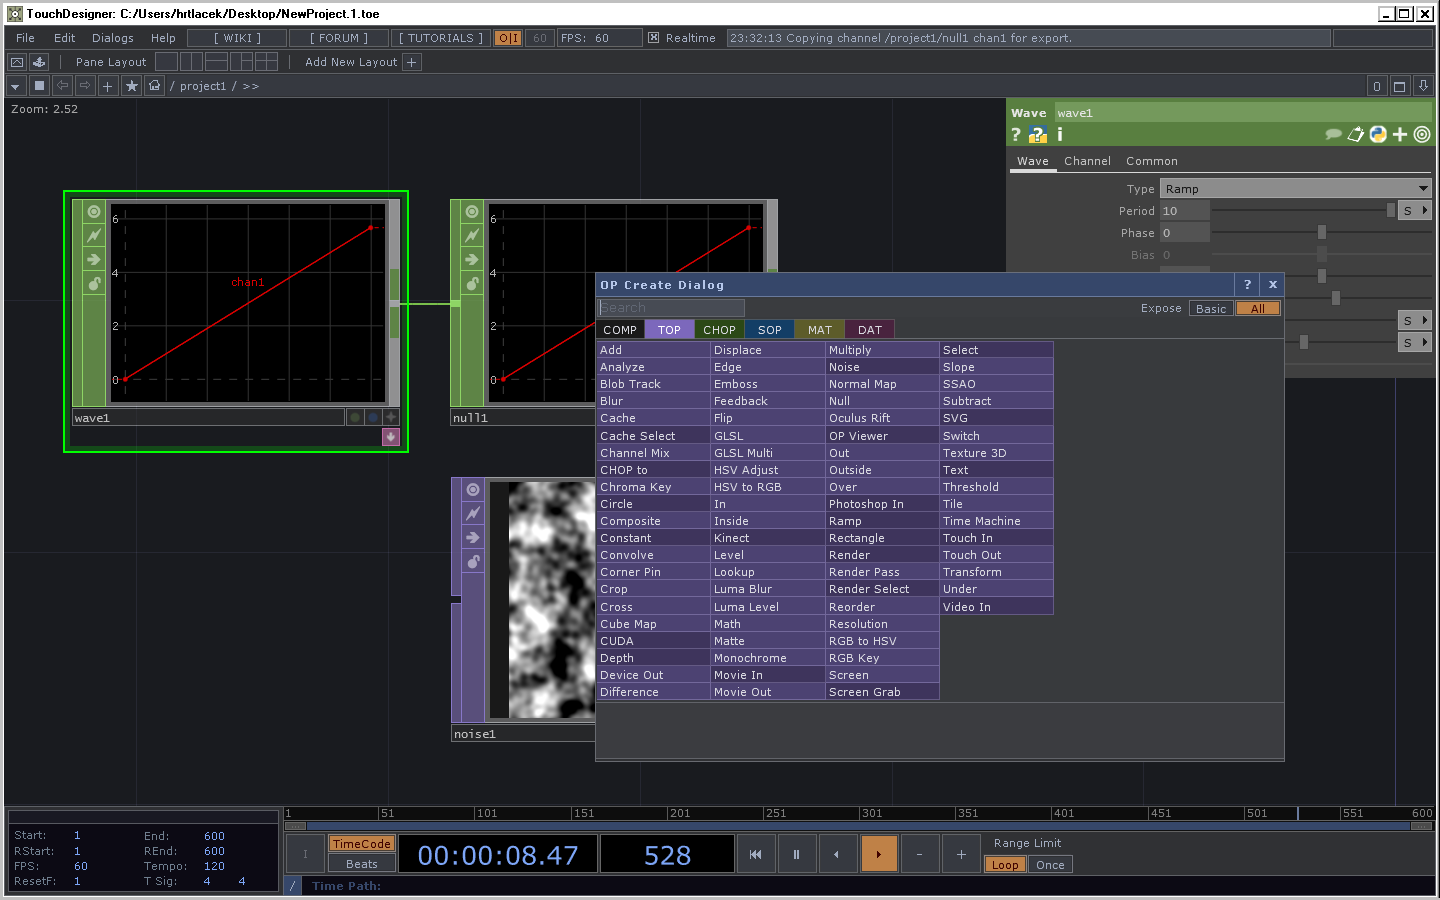
\includegraphics[width = 14cm]{img/opCreate.png}
		\caption{The OP create Dialog}
		\label{fig:opCreate}
	\end{center}
\end{figure}



We can connect \OPs by clicking at outputs and inputs of \OPs. We can only connect \OPs that are in the same \textit{family}, so \TOPs with \TOPs and \CHOPs with \CHOPs\footnote{There are ways to convert between families though, and \COMPs can have inputs whose family we can define}. We can disconnect \OPs by right-clicking at the cord and choosing \verb|disconnect| or by clicking at the inlet of the connected \OP and dragging away to an empty area.
\begin{framed}
	If we look closely at the OP Create Dialog, we can see that some of the \OPs are colored more dark and others are more light. The darker ones are \textit{generators}, so they produce data, the lighter ones are called \textit{filters} so they process data, and need input.

\end{framed}

Let's have a quick look at the header of the parameter dialog: The header section in the parameter dialog displays the type and name of the operator and provides a number of buttons for basic operations as described below. The background color of the parameter header indicates the operator's family type.

\begin{figure}[H]
	\begin{center}
		
\includegraphics[width = 14cm]{img/ParameterHeader.png}
		\caption{Parameter Dialog Header}
		\label{fig:parHeader}
	\end{center}
\end{figure}




Top Section
\begin{itemize}
	\item OP Type (Geometry \COMP in this case)
	\item OP Name
\end{itemize}

Bottom Section
\begin{itemize}
	\item Operator Help
	\item Python Class Help
	\item Operator Info
	\item Comment
	\item Clipboard
	\item Python/Tscript Operator Language Toggle
	\item Hide/Show Default Parameters
\end{itemize}

The most important ones for us at the moment are the Operator Help, the Operator Info and the Show default Parameters buttons: \\
The operator info shows us important information about the data the Operator holds (such as resolution for \TOPs or number of vertices for \SOPs) but also displays errors if we messed up something.\\
\begin{framed}
	Usually we access the Operator info just by middle-mouse clicking on the \OP itself, instead of clicking on the operator info button. That way you always have all the info always at your fingertips.
\end{framed}

\begin{figure}[H]
	\centering
	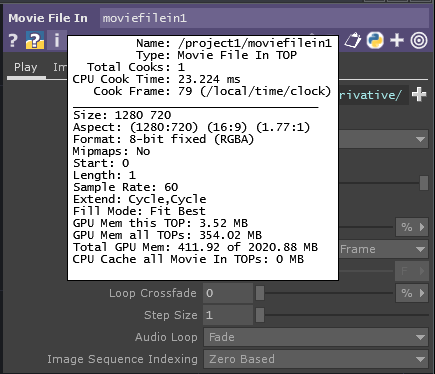
\includegraphics[width=10cm]{img/info.PNG}
	\caption[shortCaption]
	{CAPTION MISSING}
	\label{fig:label}
\end{figure}








\section{The Operator Families}
\subsection{CHOPs} % (fold)
\label{sub:CHOPs}

\begin{figure}[H]
	\begin{center}
		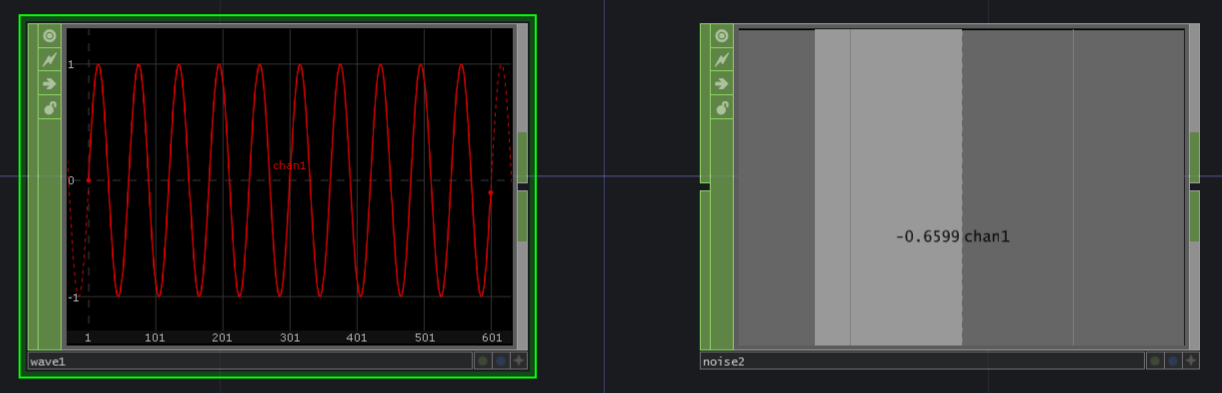
\includegraphics[width = 14cm]{img/chops.png}
		\caption{chops}
		\label{fig:chops}
	\end{center}
\end{figure}

\CHOPs are Channel Operators. Generally speaking, we could say, \CHOPs are there for movement, animation, control of parameters, control signals and streaming numeric data. For example an audio file could be loaded using the Audio File In \CHOP, an LFO\footnote{Low-Frequency Oscillator} can be created with an LFO \CHOP.  \CHOPs can contain any number of samples, and any number of channels. Also there are \CHOPs for OSC in/output, Audio in/output, MIDI, DMX, Kinect, Leap Motion and many other interfaces.

\subsection{TOPs} % (fold)
\label{sub:TOPs}

\begin{figure}[H]
	\begin{center}
		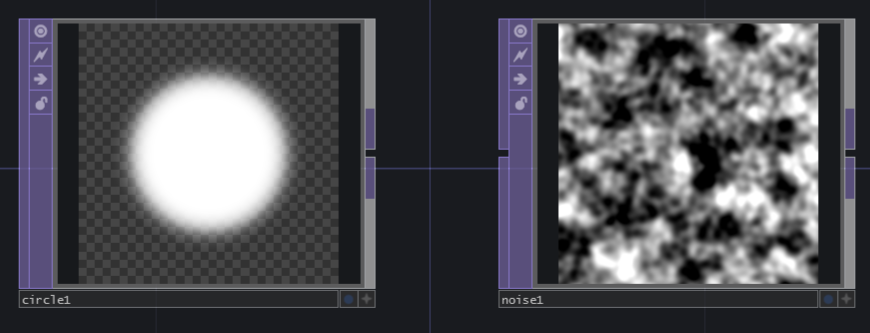
\includegraphics[width = 14cm]{img/tops.png}
		\caption{tops}
		\label{fig:tops}
	\end{center}
\end{figure}
\TOPs are Texture Operators. They hold image data, or other data in 2 dimensional/Image form. We find effects for image processing in this category. All of the Texture Operators are GPU accelerated, and therefore can be very efficient. Don't forget that images are just data, if we want to use \TOPs for working on other data than images, that's fine too, just the format has to be right. We will talk about moving between OP Families later.


\subsection{COMPs} % (fold)
\label{sub:COMPs}


\begin{figure}[H]
	\begin{center}
		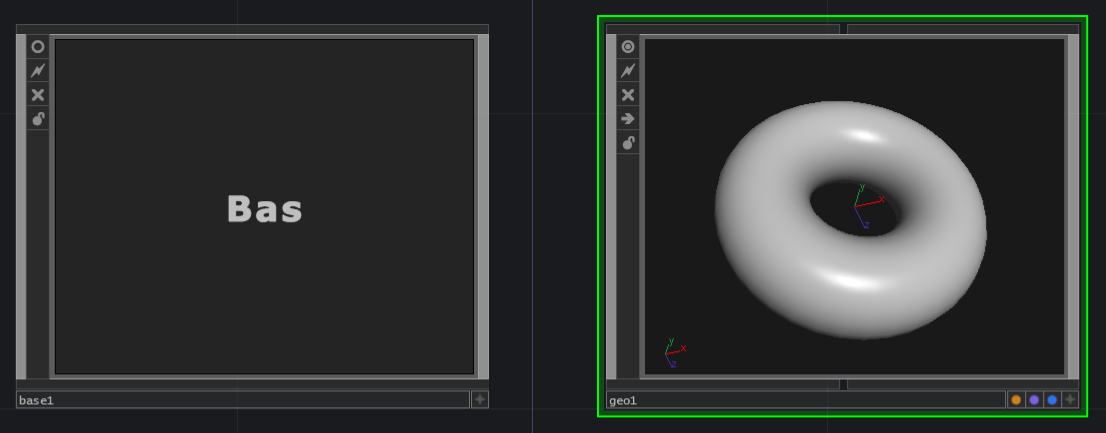
\includegraphics[width = 14cm]{img/comps.png}
		\caption{comps}
		\label{fig:comps}
	\end{center}
\end{figure}
Components, or \COMPs for short. If you come from Max/MSP or pd you can think of them as subpatchers. But in TD there are many different kinds of subpatchers.\\
\COMPs can contain other \OPs. They allow us to build up hierarchies and to organize our networks in a more tidy way. But also, there are specialized \COMPs for different purposes. If we just want to pack a network into some kind of  self-contained box we should always use a Base \COMP \index{Base Comp}. If we want our result to have a GUI also, we should rather use a Container \COMP \index{Container Comp}. Later, in chapter \ref{chap:3D_intro} we will see specialized \COMPs for 3D rendering such as a Geometry \COMP.


\subsection{SOPs} % (fold)
\label{sub:sops}

\begin{figure}[H]
	\begin{center}
		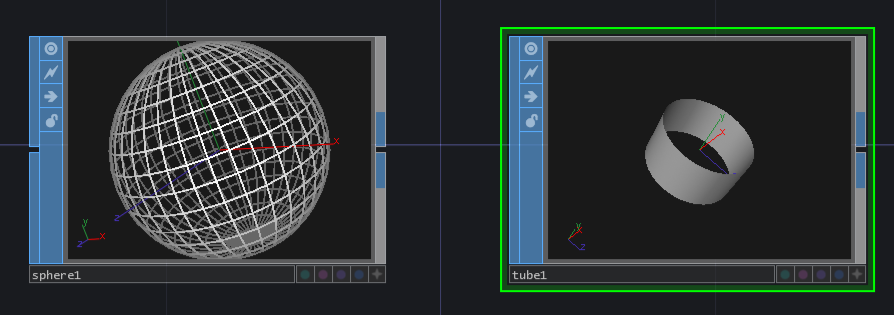
\includegraphics[width = 14cm]{img/sops.png}
		\caption{sops}
		\label{fig:sops}
	\end{center}
\end{figure}

\SOPs stands for Surface Operators. They are operators acting in 3d space. They let us model in a procedural way, transform, scale, extrude, twist and edit geometry procedurally. SOPs are processed on the CPU and then sent to a render TOP to be rendered to an image. Their CPU consumption heavily depends on the number of point they are dealing with. Also SOPs can contain different types of data: Polygons, NURBS, Meshes, primitives, bezier.

\subsection{MATs} % (fold)
\label{sub:mats}

\begin{figure}[H]
	\begin{center}
		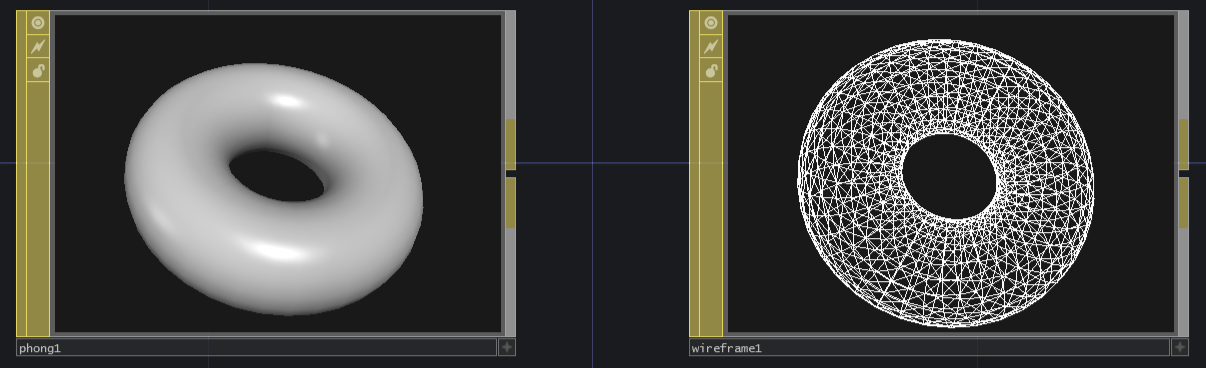
\includegraphics[width = 14cm]{img/mats.png}
		\caption{MATs}
		\label{fig:mats}
	\end{center}
\end{figure}
\MATs or Materials are used to shade geometry, so, this determines the look of our 3d objects. We are going to visit them later.

\subsection{DATs} % (fold)
\label{sub:dats}


\begin{figure}[H]
	\begin{center}
		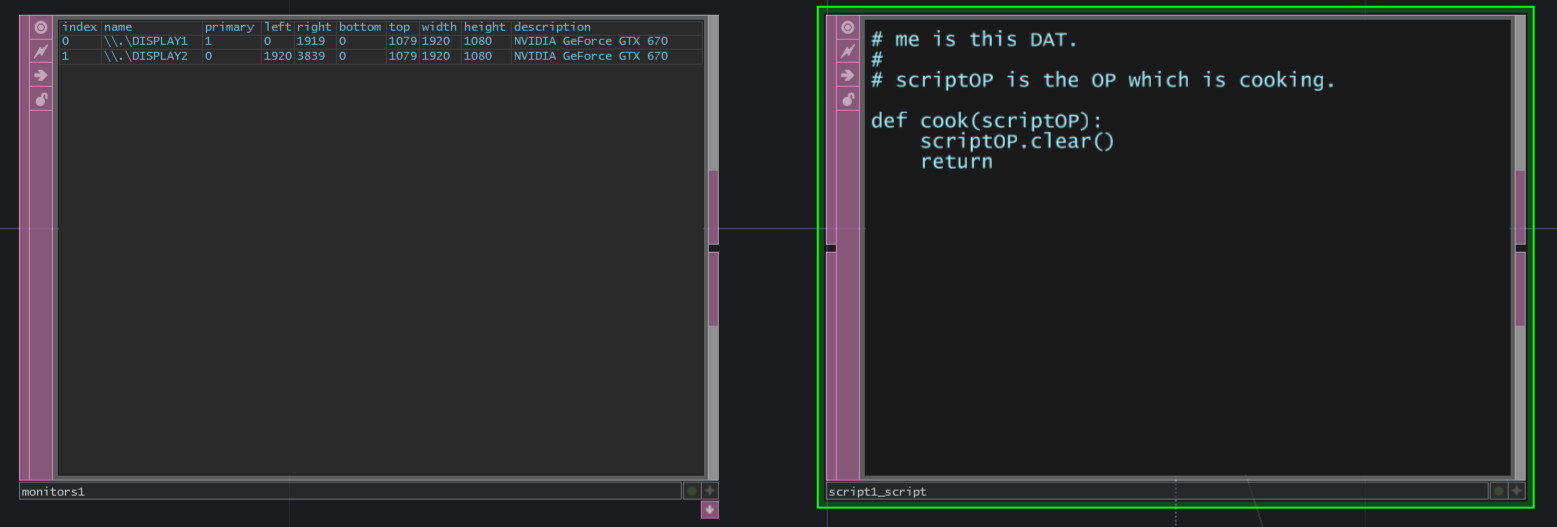
\includegraphics[width = 14cm]{img/dats.png}
		\caption{DATs}
		\label{fig:dats}
	\end{center}
\end{figure}

\DATs or Data operators, let us enter, edit and process text, code, tables and they handle incoming data as OSC, UDP, TCP/IP, MIDI etc. as well as output data using these protocols/interfaces.

\section{TOPs Introduction}

\subsection{Simple 2D Generation and Processing}

\subsubsection{Effects on Web-Cam input}
For a first simple example, let's consider \ref{fig:simple2d}. The idea is just that we take our webcam (or other video input device) and apply some effects to that stream of images.\\
As an exercise, look at the block diagram and implement it yourself in TD. The names of the Operators are identical to the labels, and remember you already know what OP family is the one for image processing, so make sure you're looking under \TOPs. Don't forget to play around with the parameters of each \OP!



  \begin{figure}[htb]
  \centering


  % \resizebox{10cm}{!}{%
  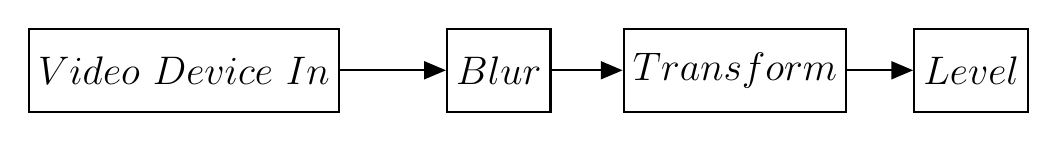
\begin{tikzpicture}[auto, thick, node distance=2.3cm, >=triangle 45]

  \draw node at (5,0) [block] (inp) {\Large$Video\ Device\ In $};
  \draw node [block, right of=inp, node distance = 4cm] (blur) {\Large$Blur$};
  \draw node [block, right of=blur, node distance = 3cm] (transform) {\Large$Transform$};
	\draw node [block, right of=transform, node distance = 3cm] (level) {\Large$Level$};
  % \draw node right of (inp) (blur) {$blur$}
  % \draw node at (5,-3) [block] (del2) {\Large$\ \ \ \ \ \ \ \ z^{-m}\ \ \ \ \ \ \ \ $};
  % \draw node at (0, -1.5) [mult] (m1) {\Large$-1$};
  % \draw node at (10, -1.5) [mult] (m2) {\Large$-1$};

  \draw[->] (inp) -- node {}(blur);
  \draw[->] (blur) -- node {}(transform);
  \draw[->] (transform) -- node {}(level);
  % \draw[->] (m2) |- node {}(del2);
  % \draw[->] (del2) -| node {}(m1);
  % \draw[->] (m1) |- node {}(del1);

  \end{tikzpicture}
  \caption{Basic real-time image processing Example.}
  \label{fig:simple2d}
\end{figure}



\begin{figure}[H]
	\begin{center}
		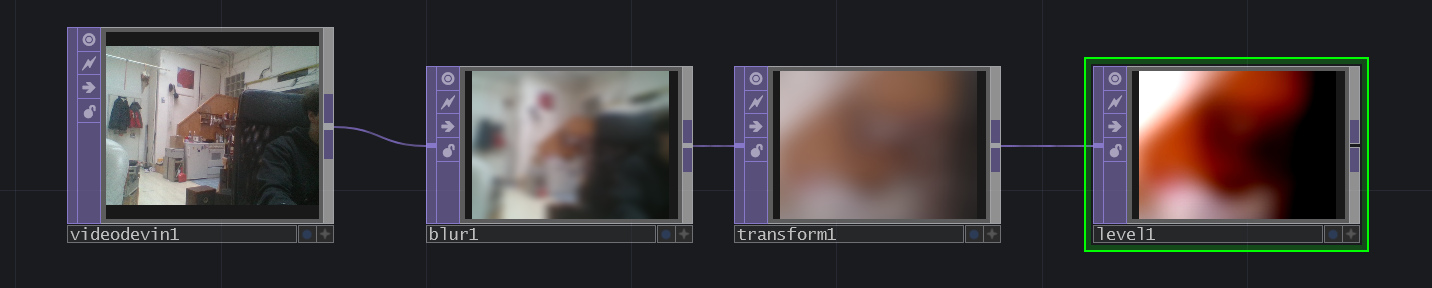
\includegraphics[width = 10cm]{img/simple2Dproc.PNG}
		\caption{The TD network representing the block diagram above.}
		\label{fig:simpleProcTD}
	\end{center}
\end{figure}


\subsubsection{Cooking and Resolution Inheritance}
Before moving on to more spectacular results such as moving images and 3D scenes, let's make sure we throughly understand how TD manages resolutions. TD in general wants to help us and wants to make clever decisions about optimization. So it will make decisions about resolutions and when it is necessary to \textbf{cook} an \OP \index{cooking}.
\begin{framed}
	The Term 'cooking' in TD refers to processing. This is not specific to \TOPs. If an \OP cooks it means it does work, consumes CPU/GPU resources and produces output data. If it does not 'cook' it just outputs static data or no data and does not consume resources (except of memory). If you look at the cords connecting the \OPs in our last example, you should see a slight animation, indicating that data is indeed flowing (because our web cam continuously delivers frames to process.) In our next example, this won't be the case.
\end{framed}
To explore resolution management, let's build a little network that produces a nice graphic with some simple shapes and some compositing. What we plan to do is depicted in Figure \ref{fig:graphicalbd}.


  \begin{figure}[H]
  \centering


  % \resizebox{10cm}{!}{%
  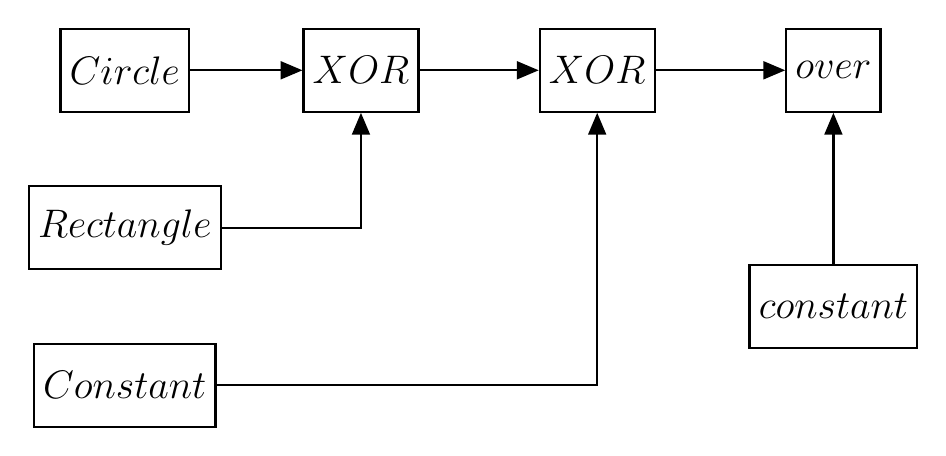
\begin{tikzpicture}[auto, thick, node distance=2.3cm, >=triangle 45]

  \draw node at (5,0) [block] (circle) {\Large$Circle $};
  \draw node [block, below of=circle, node distance = 2cm] (rectangle) {\Large$Rectangle$};
  \draw node [block, below of=rectangle, node distance = 2cm] (constant) {\Large$Constant$};

	\draw node [block, right of=circle, node distance = 3cm] (XOR) {\Large$XOR$};
	\draw node [block, right of=XOR, node distance = 3cm] (XOR2) {\Large$XOR$};
	\draw node [block, right of=XOR2, node distance = 3cm] (over) {\Large$over$};
	\draw node [block, below of=over, node distance = 3cm] (constant2) {\Large$constant$};

  % \draw node right of (inp) (blur) {$blur$}
  % \draw node at (5,-3) [block] (del2) {\Large$\ \ \ \ \ \ \ \ z^{-m}\ \ \ \ \ \ \ \ $};
  % \draw node at (0, -1.5) [mult] (m1) {\Large$-1$};
  % \draw node at (10, -1.5) [mult] (m2) {\Large$-1$};

  \draw[->] (circle) -- node {}(XOR);
  \draw[->] (rectangle) -| node {}(XOR);
  \draw[->] (XOR) -- node {}(XOR2);
  \draw[->] (constant) -| node {}(XOR2);
  \draw[->] (XOR2) -- node {}(over);

\draw[->] (constant2) -- node {}(over);

  % \draw[->] (m2) |- node {}(del2);
  % \draw[->] (del2) -| node {}(m1);
  % \draw[->] (m1) |- node {}(del1);

  \end{tikzpicture}
  \caption{Network for producing a simple geometric graphic}
  \label{fig:graphicalbd}
\end{figure}

Give it a try before looking at the screen-shot in figure \ref{fig:graphical}. The Blocks labeled $XOR$ are just \link{http://derivative.ca/wiki099/index.php?title=Composite\_TOP}{Composite} \TOPs, whose mode has been switched to the XOR operation\footnote{XOR stands for exclusive OR, a common boolean operation that will be positive if and only if \textbf{one} of the two inputs is positive. It will also be False/not positive if both of the inputs are True/Positive.}.\\
Play around with the parameters a bit, I adjusted the scale and position parameters of both the circle and the rectangle, and used the rotate parameter of the rectangle to arrive at what's depicted in Figure \ref{fig:graphical}.\\
Now let's look at the resolutions we are operating with. When you middle mouse click on the \OPs, you can see their resolutions. By default they are all at $256 \times 256$. Now that's a bit poor, so let's do something about this. All \OPs have a common page in their parameter dialog. It contains parameters common to that family of \OPs, hence the name. In figure \ref{fig:topCommon} you can see the common page of one of the \link{http://derivative.ca/wiki099/index.php?title=Composite\_TOP}{Composite} \TOPs.
\begin{figure}[H]
	\centering
	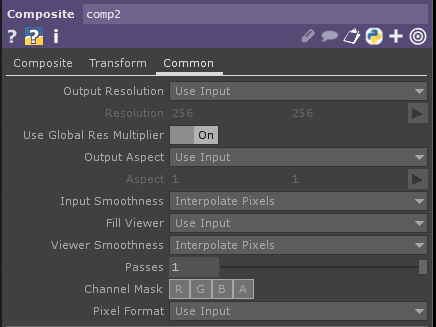
\includegraphics[width=10cm]{img/TOPcommonPars.PNG}
	\caption[TOP common parameters]
	{TOP common pars}
	\label{fig:topCommon}
\end{figure}


Since this \OP is a \glqq{}filter\grqq{}, so it has an input, it has the option to use its input to determine the output resolution. This will be default for all filter \OPs.\\
If you now go to the \refTOP{Circle}, you will find it has a resolution parameter that is set to $256 \times 256$. Try changing it to $1024\times1024$. You will see, if you zoom in a bit, the resolution is quite a bit better, for the circle at least.\\
The composite \OPs can take multiple input signals, so which resolution should they take?\\
By default, always the last \OP's resolution is used. So if you also change the resolution of the \refTOP{Rectangle}, the two \refTOP{Constant}s you will find the whole network is running at a higher resolution.



\begin{figure}[H]
	\centering
	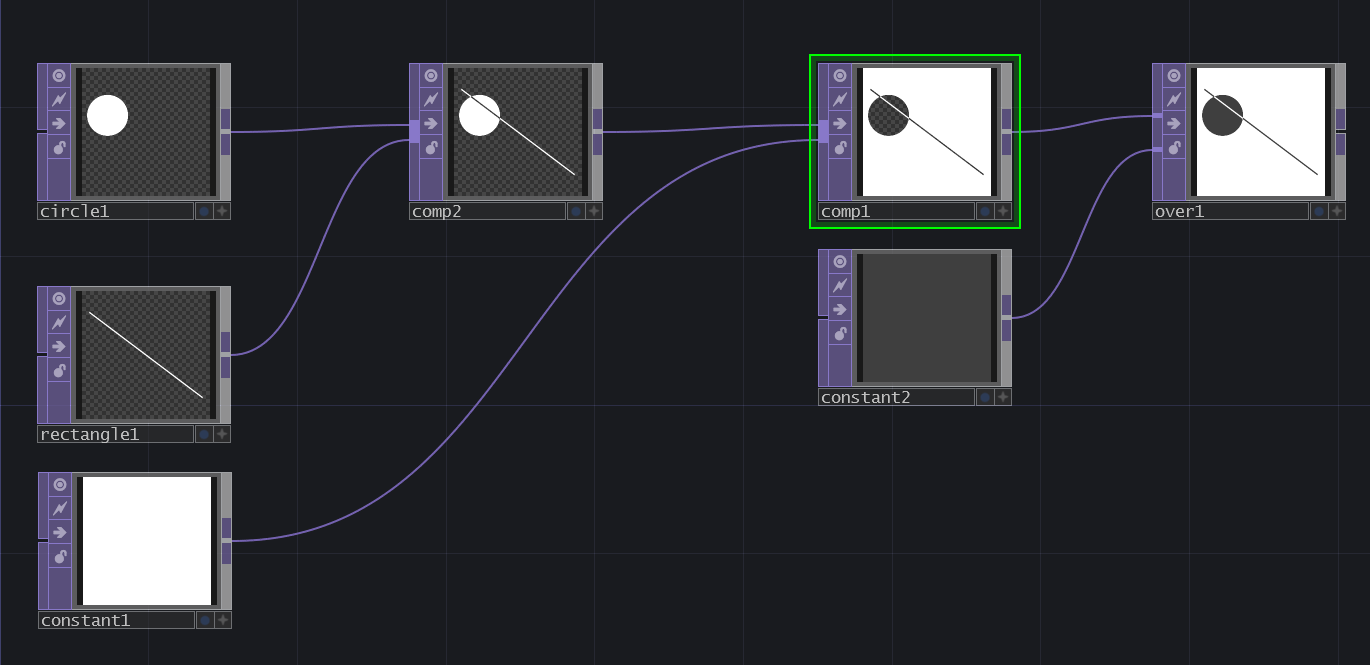
\includegraphics[width=\textwidth]{img/graphical.PNG}
	\caption[shortCaption]
	{CAPTION MISSING}
	\label{fig:graphical}
\end{figure}


\noindent\rule{12cm}{0.4pt}
\\
	\textbf{Exercise:}
	The last example was inspired by \link{http://derivative.ca/events/2018/BlokArtwork/}{this}. Try to imitate the other examples there!
\\
\noindent\rule{12cm}{0.4pt}



\subsubsection{TOP common page}

Looking at Figure \ref{fig:topCommon}, you can see a lot of parameters that rather seem technical, such as resolution and bit depth. Don't be fooled, some of these can be really interesting from an artistic/creative point of view. As an example we will explore the parameter \texttt{Channel Mask}. For a full description of all parameters, please look at the \link{http://www.derivative.ca/wiki099/index.php?title=TOP\_Generator\_Common\_Page}{TOP Generator Common Page Wiki entry} or the \link{http://www.derivative.ca/wiki099/index.php?title=TOP\_Filter\_Common\_Page}{TOP Filter Common Page Wiki entry}.\\
Let's put a \refTOP{Transform} after our current network. Use its parameters to move the whole image slightly to the right. After that, go to the \refTOP{Transform}'s Common Page and under \texttt{Channel Mask}, switch off the button with the Label 'R'. This deactivates the \TOP's effect for the red channel. The result is a commonly used effect:

\begin{figure}[H]
	\centering
	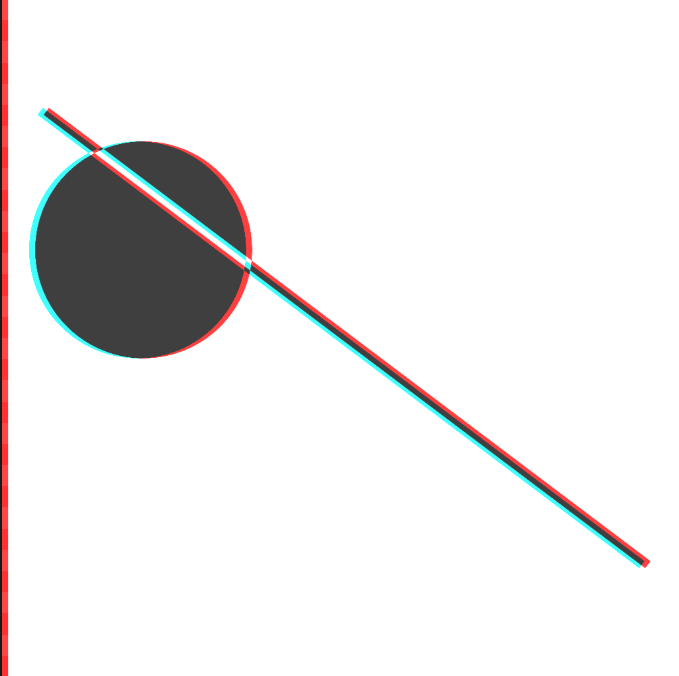
\includegraphics[width=7cm]{img/R_shift.PNG}
	\caption[All but the red channel Shifted]
	{All but the red channel Shifted}
	\label{fig:label}
\end{figure}


\subsection{Simple Output}
So we did process some live input and observed the results by just looking at the \OPs viewers. But in reality, we need some kind of output, be it saving an image or video to disk, be it full-screen output to one or more projectors, LED walls, or maybe we output DMX to control lights.\\
As you can see, different situations demand different output techniques, but mainly to keep us motivated, let's just record a quick movie and try out full-screen output to one monitor.\\

\subsubsection{Recording Movies and Images}

Let's keep thing simple for now. Use our previous example and put down a \refTOP{Movie\_File\_Out}. In its parameters, you can choose if you want to record an image or a movie, you can choose the location where the file will be saved and other parameters such as compression.\\
Just switch on record and switch it off again when you want to finish your recording.\\
TD allows us to also record 'offline' so it wont loose any frames and takes time to render frames. This is especially important if we built a network that exceeds the real-time performance of our machine. We will get into this topic at a later point of this document.

\subsubsection{Full-Screen Output}
\index{Window COMP}
For this topic, we will build a very simple new network, but finally one with some movement. When looking at the block diagram in Figure \ref{fig:outputDispl} beware that our block diagrams are slowly going to get more abstract and less explicit. For example there is no $Output$ \TOP\footnote{There is an Out \TOP, but it isn't meant here and we are going to see what it does soon.}. What's meant here is that this is going to be the output of our network, going to the screen. The network is supposed to load and play a movie file and distort it using the \refTOP{Displace}. This should then be output using a Window \COMP.

	\begin{figure}[H]
	\centering


	% \resizebox{10cm}{!}{%
	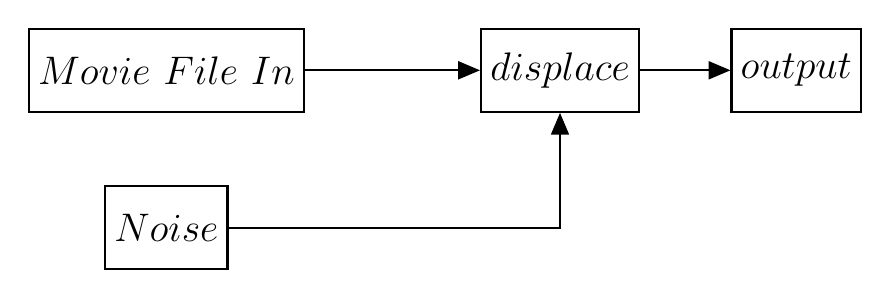
\begin{tikzpicture}[auto, thick, node distance=2.3cm, >=triangle 45]

	\draw node at (5,0) [block] (movie) {\Large$Movie\ File\ In $};
	\draw node [block, below of=movie, node distance = 2cm] (noise) {\Large$Noise$};
	\draw node [block, right of=movie, node distance = 5cm] (displace) {\Large$displace$};

	\draw node [block, right of=displace, node distance = 3cm] (output) {\Large$output$};
	% \draw node [block, right of=XOR, node distance = 3cm] (XOR2) {\Large$XOR$};
	% \draw node [block, right of=XOR2, node distance = 3cm] (over) {\Large$over$};
	% \draw node [block, below of=over, node distance = 3cm] (constant2) {\Large$constant$};

  % \draw node right of (inp) (blur) {$blur$}
  % \draw node at (5,-3) [block] (del2) {\Large$\ \ \ \ \ \ \ \ z^{-m}\ \ \ \ \ \ \ \ $};
  % \draw node at (0, -1.5) [mult] (m1) {\Large$-1$};
  % \draw node at (10, -1.5) [mult] (m2) {\Large$-1$};

  \draw[->] (movie) -- node {}(displace);
  \draw[->] (noise) -| node {}(displace);
  \draw[->] (displace) -- node {}(output);
%   \draw[->] (constant) -| node {}(XOR2);
%   \draw[->] (XOR2) -- node {}(over);

% \draw[->] (constant2) -- node {}(over);

  % \draw[->] (m2) |- node {}(del2);
  % \draw[->] (del2) -| node {}(m1);
  % \draw[->] (m1) |- node {}(del1);

  \end{tikzpicture}
  \caption{Network for producing a simple geometric graphic}
  \label{fig:outputDispl}
\end{figure}

Build up the network and maybe lower the Displace \TOP's \texttt{Displace Weight} parameter to about $0.06$ (both the x and the y value) to make the effect less extreme. Also switch off \texttt{Monochrome} of the \refTOP{Noise}.\\
Finally enter the following expression into the Noise \TOP's Translate z parameter as depicted in \ref{fig:expressionNoiseTOP}: \texttt{absTime.frame/100}.

\begin{framed}
	What does the expression \texttt{absTime.frame/100} mean? \texttt{absTime.frame} always returns the current absolute frame, so an integer that stands for the current frame number since we started TD. It is an ever increasing number.\\
	We can use that to translate the Noise. What does that mean? Noise is a collection of quasi-random values. These values are computed along a domain, and this domain can be shifted. Translate the noise \TOP's output in X or Y and you will immediately see that it just 'moves' the image left/right or up/down. Moving in Z moves in another dimension, seemingly creating a \textbf{continuous} set of new random values. Continuous means that the image does not 'jump', it gradually changes, which is often what we want.\\
	The division, so \texttt{/100} just slows down this behavior since that movement happens 100 times slower.
\end{framed}

\begin{figure}[H]
	\centering
	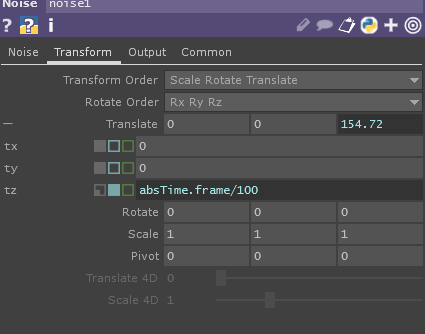
\includegraphics[width=10cm]{img/noiseTopExpr.PNG}
	\caption[An expression in the Transform parameter of the Noise \TOP.]
	{Expression in Noise TOP}
	\label{fig:expressionNoiseTOP}
\end{figure}



\begin{figure}[H]
	\centering
	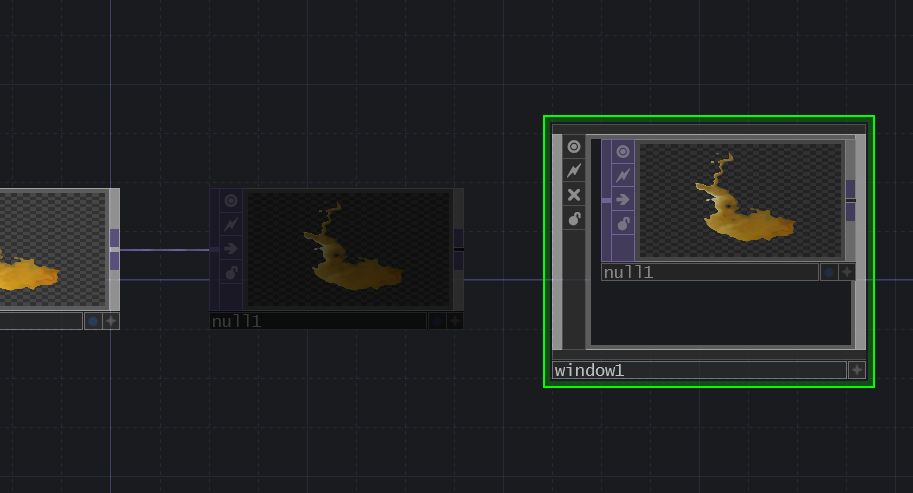
\includegraphics[width=\textwidth]{img/dragOnWindow.PNG}
	\caption[shortCaption]
	{CAPTION MISSING}
	\label{fig:label}
\end{figure}

\begin{figure}[H]
	\centering
	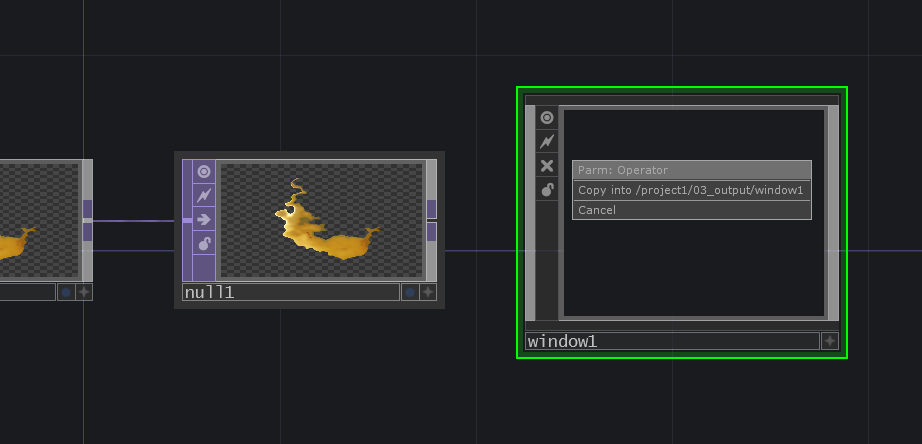
\includegraphics[width=\textwidth]{img/dragMenu.PNG}
	\caption[shortCaption]
	{CAPTION MISSING}
	\label{fig:label}
\end{figure}

\begin{figure}[H]
	\centering
	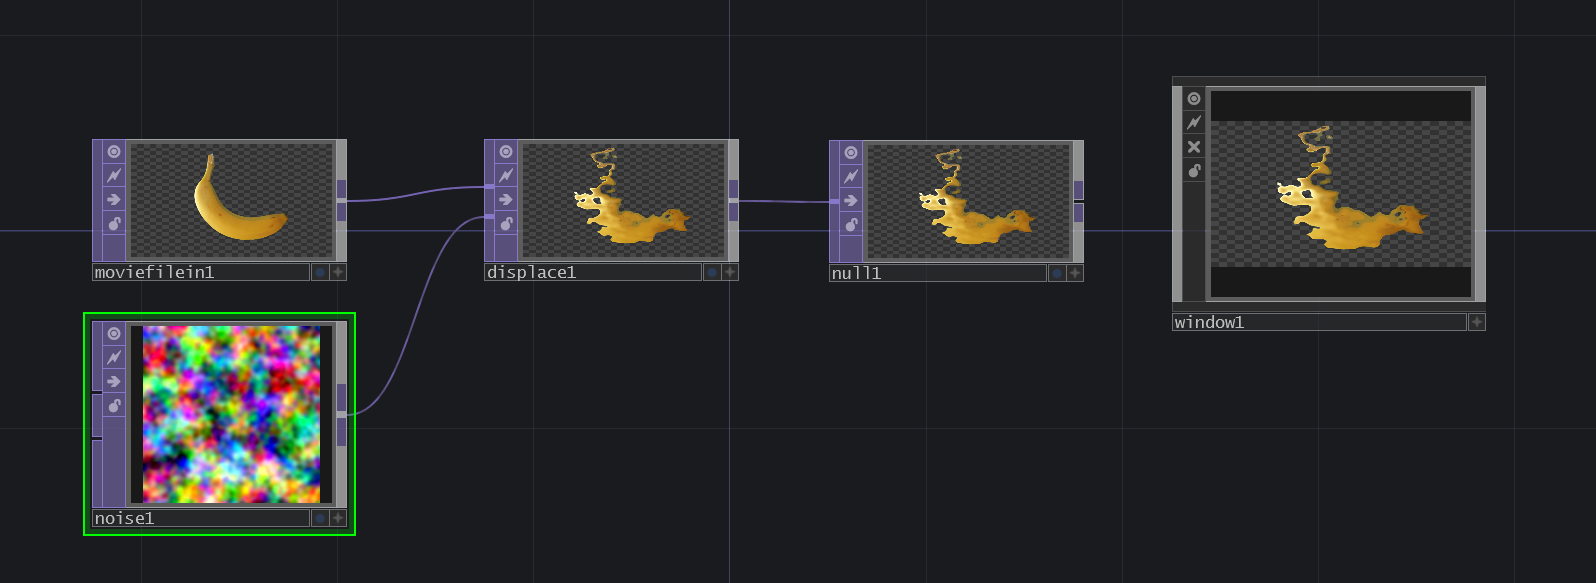
\includegraphics[width=\textwidth]{img/outputToWindow.PNG}
	\caption[shortCaption]
	{CAPTION MISSING}
	\label{fig:label}
\end{figure}




\begin{figure}[H]
	\centering
	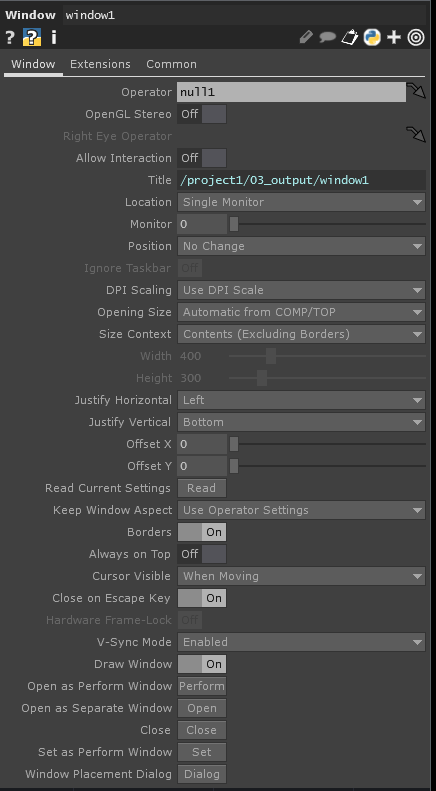
\includegraphics[width=8cm]{img/windowCompPars.PNG}
	\caption[shortCaption]
	{CAPTION MISSING}
	\label{fig:label}
\end{figure}


\section{CHOPs Introduction}
\begin{itemize}
\item Audio Device In \CHOP
\item Audio Device Out \CHOP
\item Audio File In \CHOP
\item Audio Filter \CHOP
\item Analysis \CHOP
\end{itemize}

\subsection{CHOP exporting}
\index{CHOP Exporting}


\subsection{Audio Analysis}
\index{Audio Analysis}

If we want to control the appearance of something, be it geometry/visuals or dmx/lights by an audio signal, we generally use the structure depicted in Figure \ref{fig:audioAnalysis2}.


	\begin{figure}[H]
	\centering


	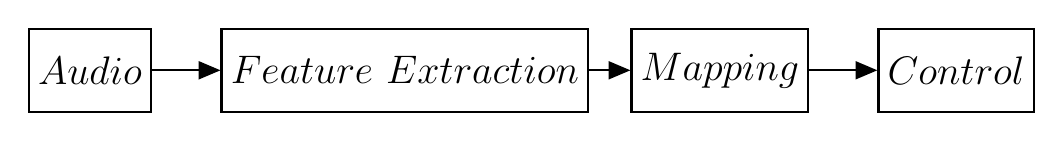
\begin{tikzpicture}[auto, thick, node distance=2.3cm, >=triangle 45]

	\draw node at (5,0) [block] (audio) {\Large$Audio $};
	\draw node [block, right of=audio, node distance = 4cm] (fe) {\Large$Feature\ Extraction$};

	\draw node [block, right of=fe, node distance = 4cm] (mapping) {\Large$Mapping$};

	\draw node [block, right of=mapping, node distance = 3cm] (output) {\Large$Control$};

  \draw[->] (audio) -- node {}(fe);
  \draw[->] (fe) -- node {}(mapping);
  \draw[->] (mapping) -- node {}(output);

  \end{tikzpicture}
  \caption{Using Audio to control visual parameters.}
  \label{fig:audioAnalysis2}
\end{figure}


Audio digital signals are numbers. For a stereo signal, we get always 2 number in any moment of time. Also we typically get 44100 numbers per second per channel. So we get a lot of numbers, be it from a microphone, a sound card input or a file. \\
These numbers themselves are not directly suitable to control something video related.
Let's say we ignored on channel, so we get 44100 numbers per second. Let's assume we take these numbers to control the brightness of some video. First of all we will miss most of the action since our screens produce only 60 images per second if we are lucky. So we miss most of the 44100 values per second. And if we have really bad luck, these 60 images are all produced when the audio wave is passing through 0 or negative (audio signals typically move between -1 and 1). So our audio input could be really loud and our output could stay dark.\\

So we need some idea \textbf{what} we want to visualize. Loudness? The loudness of the bassdrum? The whole spectrum? We could think of many things and we will need some way to measure these. This process of measuring something about the audio is called \textit{Feature Extraction}. For a simple measure of loudness we could use the \textit{RMS}.\\

The next step might be to map this extracted measurement to a parameter, let's say the sized of a sphere. The linear RMS will range between 0 and 1. Now if we don't want the sphere to be 0 when the audio is silent, we will need to apply a \textit{mapping}. This just means that we take our RMS and by multiplication and addition, bring it in another range, for example we could add 1. Then our sphere will have a size of 1 in case of silence and double the size in case of maximal input RMS. In TouchDesigner, the Math \CHOP helps us a lot with this process. On its second page it offers us to map one range to another. We just have to tell it our input and output range and it does the remapping.\\
Beware that we could also apply a non-linear mapping, for example squaring or thresholding. We could look if the input is higher than some particular value and only then doe a certain action.




\subsection{Simple Spectrum Display}
\begin{figure}[H]
	\centering
	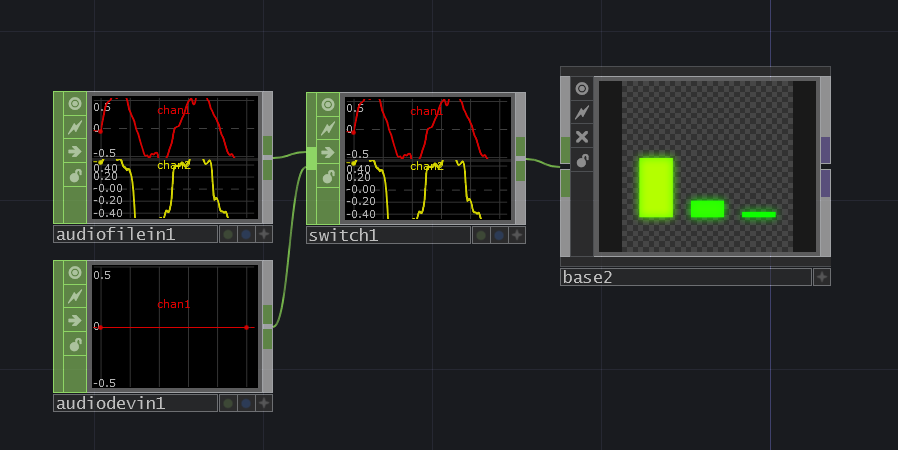
\includegraphics[width=\textwidth]{img/simpleSpecOverview.PNG}
	\caption[shortCaption]
	{CAPTION MISSING}
	\label{fig:label}
\end{figure}

\begin{figure}[H]
	\centering
	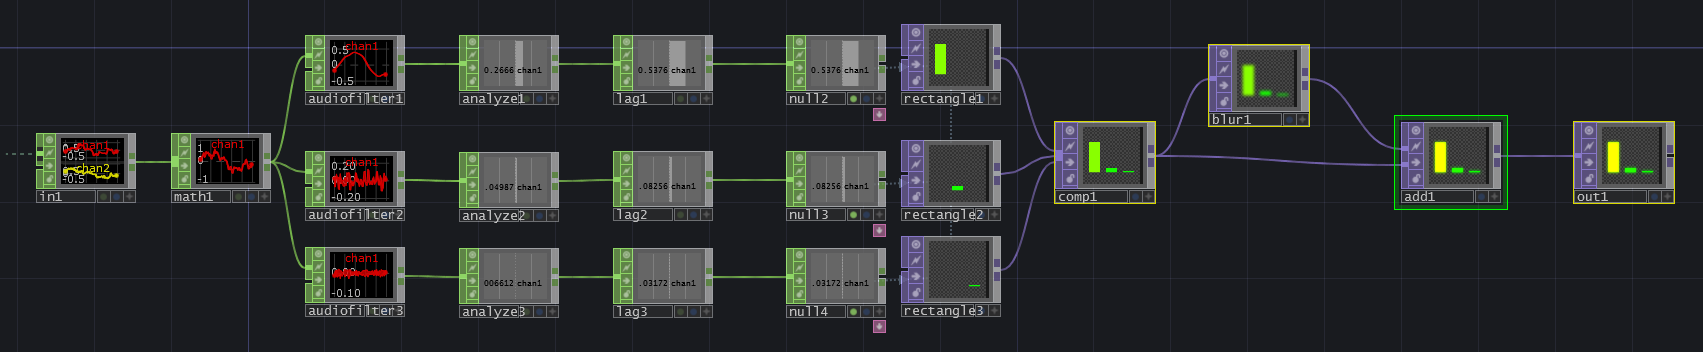
\includegraphics[width=\textwidth]{img/simpleSpec_inside.PNG}
	\caption[shortCaption]
	{CAPTION MISSING}
	\label{fig:label}
\end{figure}


%!TEX root = main.tex
%=================TD functions==================
\def\boldcommandlist{\@elt OP,\@elt OPs,}
\def\@elt#1,{%
 \expandafter\def\csname#1\endcsname{\textbf{#1}\xspace}
}
\boldcommandlist

\def\topColorList{\@elt TOP,\@elt TOPs,}
\def\@elt#1,{%
 \expandafter\def\csname#1\endcsname{\textcolor{TOP}{\textbf{#1}}\xspace}
}
\topColorList

\def\chopColorList{\@elt CHOP,\@elt CHOPs,}
\def\@elt#1,{%
 \expandafter\def\csname#1\endcsname{\textcolor{CHOP}{\textbf{#1}}\xspace}
}
\chopColorList

\def\sopColorList{\@elt SOP,\@elt SOPs,}
\def\@elt#1,{%
 \expandafter\def\csname#1\endcsname{\textcolor{SOP}{\textbf{#1}}\xspace}
}
\sopColorList

\def\datColorList{\@elt DAT,\@elt DATs,}
\def\@elt#1,{%
 \expandafter\def\csname#1\endcsname{\textcolor{DAT}{\textbf{#1}}\xspace}
}
\datColorList

\def\matColorList{\@elt MAT,\@elt MATs,}
\def\@elt#1,{%
 \expandafter\def\csname#1\endcsname{\textcolor{MAT}{\textbf{#1}}\xspace}
}
\matColorList


\def\compColorList{\@elt COMP,\@elt COMPs,}
\def\@elt#1,{%
 \expandafter\def\csname#1\endcsname{\textcolor{COMP}{\textbf{#1}}\xspace}
}
\compColorList

\def\redcommandlist{\@elt missingImage,\@elt testThis,}
\def\@elt#1,{%
 \expandafter\def\csname#1\endcsname{\textcolor{red}{\textbf{#1}}\xspace}
}
\redcommandlist

%===============================================

\chapter{Lecture 2, 3D Rendering}
\label{chap:3D_intro}

\section{Notes}
TOPs:\\
\begin{itemize}
  \item feedback + scale
  \item simple reaction-diffusion
\end{itemize}
Panel COMP -> Make TOP network interactive

3d Render Setup

Classic torus + noise

Panes: 3d viewport

feedback+CircleSOP+noise SOP+Panel interaction

CHOP to SOP (oscilloscope/Spectroscope)




converting between OPs\\
render setup\\
SOPs:\\
\begin{itemize}
  \item Torus
  \item Grid
  \item Sphere
  \item Noise
  \item facet
  \item transform
\end{itemize}




\begin{center}
\begin{figure}[h!]
\tikzset{concept/.append style={fill={none}}}
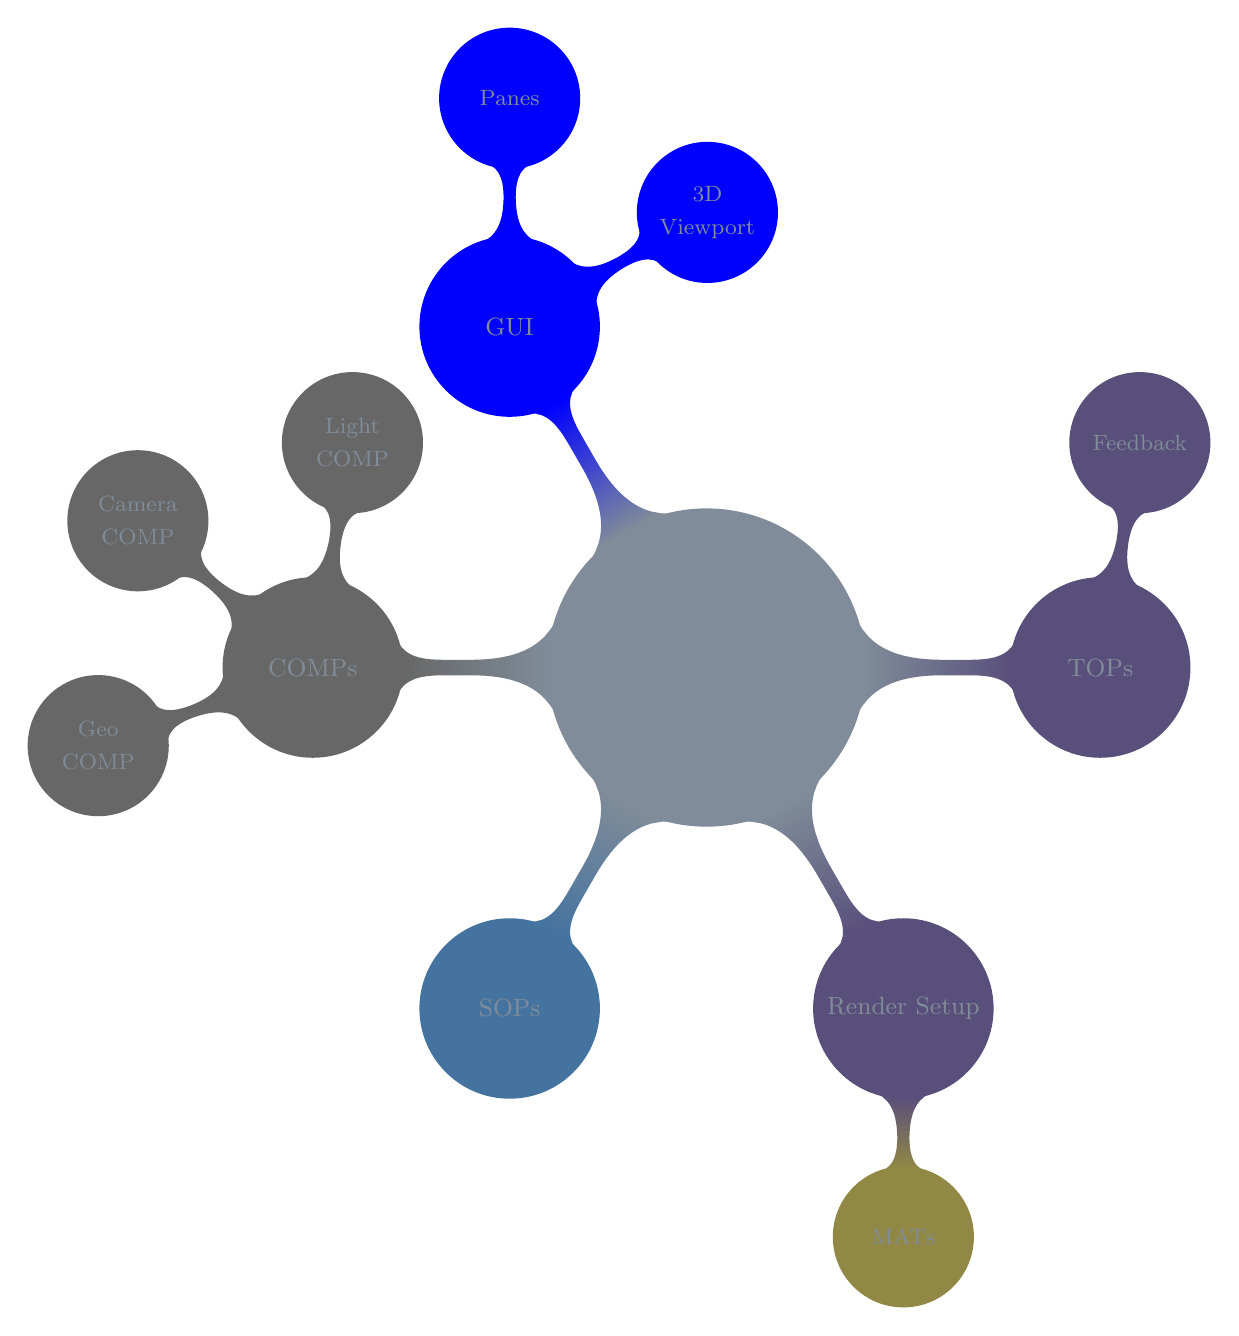
\begin{tikzpicture}
  \path[mindmap,concept color=textStd,text=textStd]
    node[concept] {3D}
    [clockwise from=0]
    child[concept color=TOP] {
      node[concept] (dats) {TOPs}
      [clockwise from=80]child[concept]{node[concept] {Feedback}}
    }
    child[concept color=TOP] { node[concept] {Render Setup}
        [clockwise from=270] child[concept color=MAT] { node[concept] {MATs}}
    }
    child[concept color=SOP] {
      node[concept] {SOPs}
      [clockwise from=90]
    }
    % child[concept color=CHOP] {
    %   node[concept] (dats) {Audio Analysis}
    %   [clockwise from=-30]
    % }
    child[concept color=COMP] { node[concept] (pm){COMPs}
        [clockwise from=200] child[concept]{node[concept] {Geo COMP}}
        child[concept]{node[concept] {Camera COMP}}
        child[concept]{node[concept] {Light COMP}}
        }
    child[concept color=blue] { node[concept] {GUI}
        [clockwise from=90] child[concept]{node[concept] {Panes}}
        child[concept]{node[concept] {3D Viewport}}
    };


\end{tikzpicture}
\caption{Lecture Contents}
\end{figure}
\end{center}


\newpage
\section{More TOPs}

\subsection{Feedback Networks}

\subsubsection{Reaction-diffusion}
\link{http://www.karlsims.com/rd.html}{Karl Sims Tutorial}

\begin{figure}[H]
  \centering
  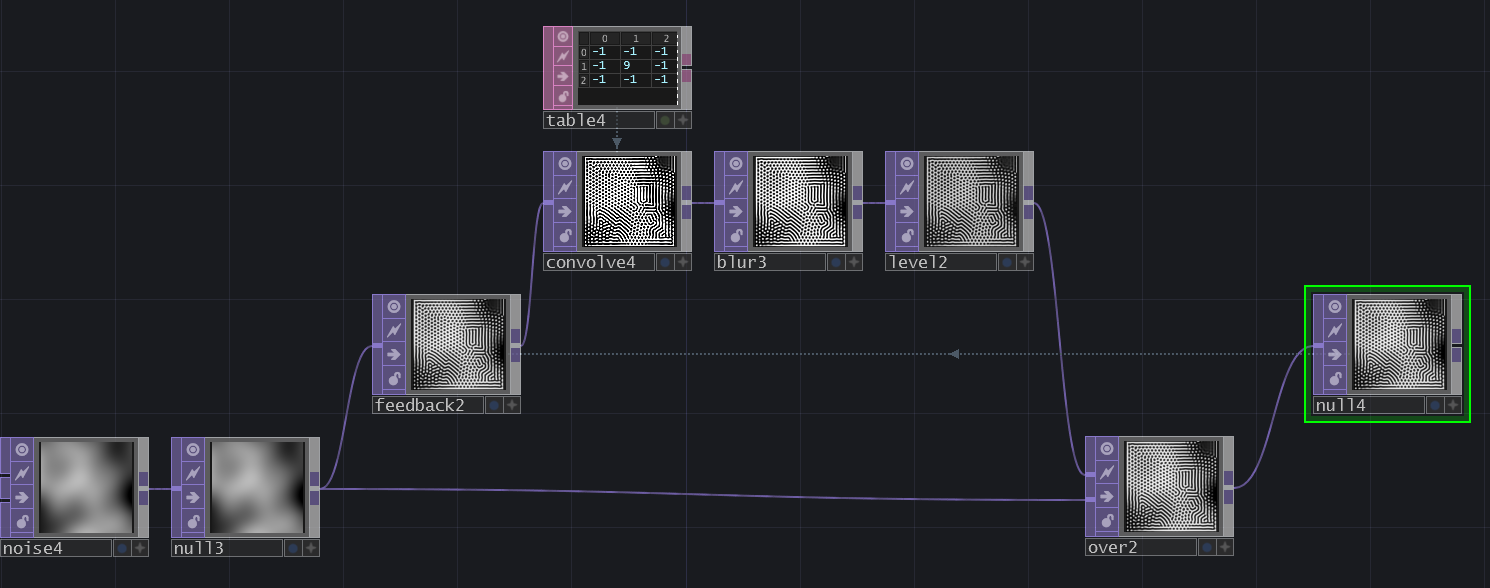
\includegraphics[width=\textwidth]{img/reactDiffuse.PNG}
  \caption[shortCaption]
  {CAPTION MISSING}
  \label{fig:label}
\end{figure}


\section{Basic Render Setup}
\index{Render Setup}
For a minimal 3D render setup we need 4 things:
\begin{itemize}
	\item Geometry \COMP
	\item Camera \COMP
	\item Light \COMP
	\item Render \TOP
\end{itemize}

\begin{figure}[H]
  \centering
  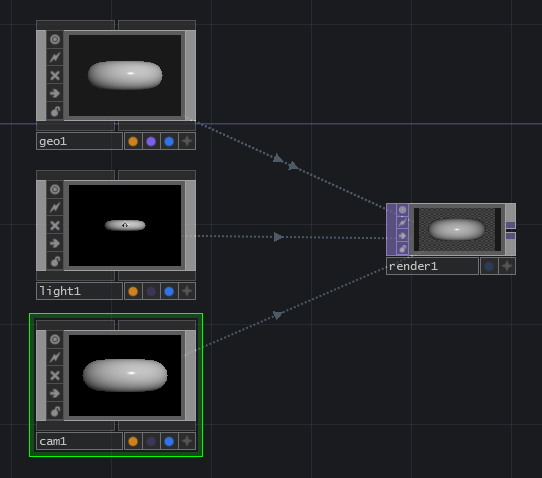
\includegraphics[width=10cm]{img/rendreSetup.PNG}
  \caption[render setup]
  {A very basic 3D rendering setup}
  \label{fig:label}
\end{figure}

\subsection{SOP Flags}


\subsection{MATs}




\subsection{Basic SOP manipulation}

\begin{figure}[H]
  \centering
  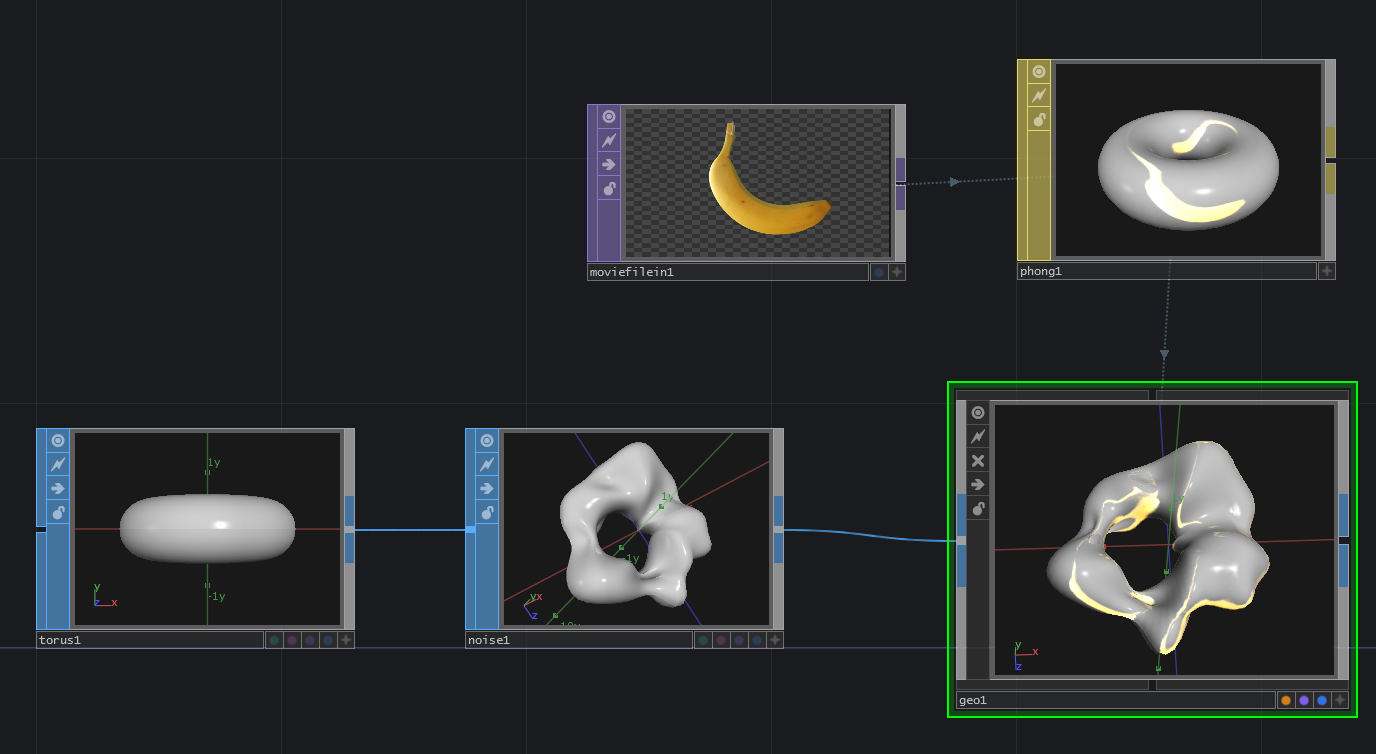
\includegraphics[width=\textwidth]{img/noise3D.PNG}
  \caption[shortCaption]
  {CAPTION MISSING}
  \label{fig:label}
\end{figure}


\subsection{The data inside a SOP}
\begin{figure}[H]
  \centering
  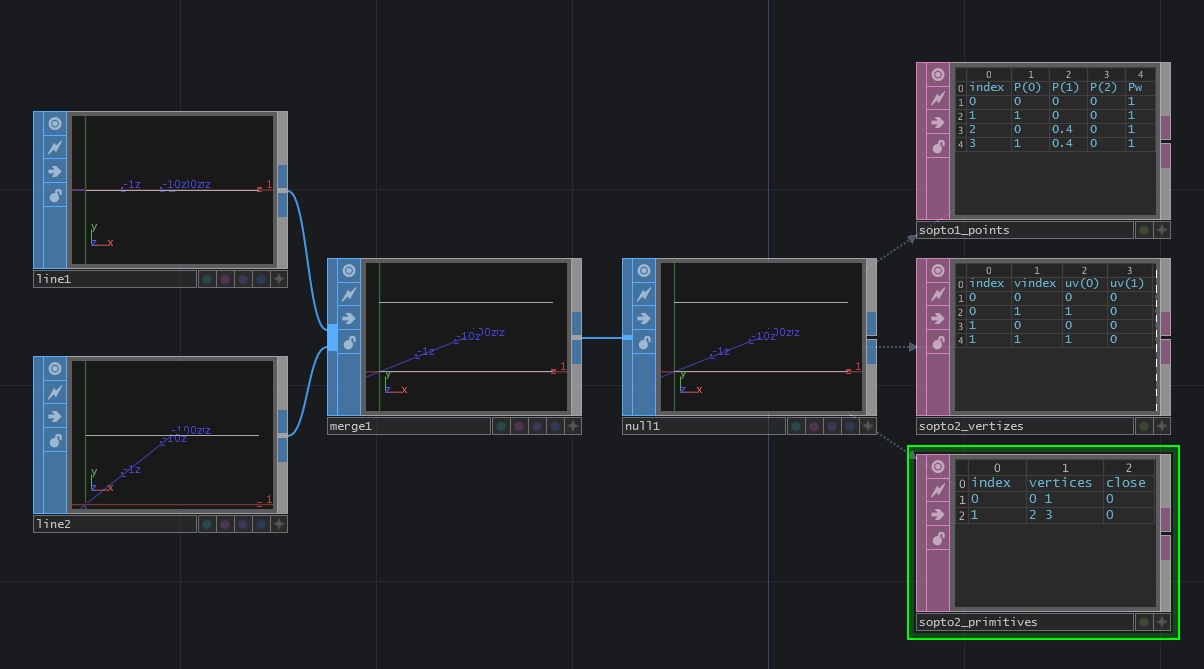
\includegraphics[width=\textwidth]{img/sopToDat.PNG}
  \caption[shortCaption]
  {CAPTION MISSING}
  \label{fig:label}
\end{figure}


\begin{framed}
  What's the difference between a point and a vertex? To quote the \link{http://derivative.ca/wiki099/index.php?title=Point}{TouchDesigner wiki}:\\
  Each SOP has a list of Points. Each point has
  \begin{itemize}
     \item an XYZ 3D position value
     \item Other optional standard attributes like RGB color, alpha, texture UV and W, Normal XYZ.
     \item user-defined attributes.
   \end{itemize}
Each polygon is defined by a vertex list, which is a list of point numbers.

So a point describes a position in 3D. A vertex is a building block of geometry that references a point. One point can be referenced by multiple vertizes.

\end{framed}
%!TEX root = main.tex
%=================TD functions==================
\def\boldcommandlist{\@elt OP,\@elt OPs,}
\def\@elt#1,{%
 \expandafter\def\csname#1\endcsname{\textbf{#1}\xspace}
}
\boldcommandlist

\def\topColorList{\@elt TOP,\@elt TOPs,}
\def\@elt#1,{%
 \expandafter\def\csname#1\endcsname{\textcolor{TOP}{\textbf{#1}}\xspace}
}
\topColorList

\def\chopColorList{\@elt CHOP,\@elt CHOPs,}
\def\@elt#1,{%
 \expandafter\def\csname#1\endcsname{\textcolor{CHOP}{\textbf{#1}}\xspace}
}
\chopColorList

\def\sopColorList{\@elt SOP,\@elt SOPs,}
\def\@elt#1,{%
 \expandafter\def\csname#1\endcsname{\textcolor{SOP}{\textbf{#1}}\xspace}
}
\sopColorList

\def\datColorList{\@elt DAT,\@elt DATs,}
\def\@elt#1,{%
 \expandafter\def\csname#1\endcsname{\textcolor{DAT}{\textbf{#1}}\xspace}
}
\datColorList

\def\matColorList{\@elt MAT,\@elt MATs,}
\def\@elt#1,{%
 \expandafter\def\csname#1\endcsname{\textcolor{MAT}{\textbf{#1}}\xspace}
}
\matColorList


\def\compColorList{\@elt COMP,\@elt COMPs,}
\def\@elt#1,{%
 \expandafter\def\csname#1\endcsname{\textcolor{COMP}{\textbf{#1}}\xspace}
}
\compColorList

\def\redcommandlist{\@elt missingImage,}
\def\@elt#1,{%
 \expandafter\def\csname#1\endcsname{\textcolor{red}{\textbf{#1}}\xspace}
}
\redcommandlist

%===============================================

\chapter{Lecture 3}

\section{Notes}

\begin{itemize}
	\item \SOPs explanations: Transform, Merge, Copy, Subdivide, Group
	\item Geometry Types, SOP to \DAT for inspection
	\item Panel Interaction + Generative Design Example
	\item Instancing, SOP to \CHOP
	\item Oscilloscope
	\item Trail \CHOP + instancing


\end{itemize}


\begin{figure}[H]
	\centering
	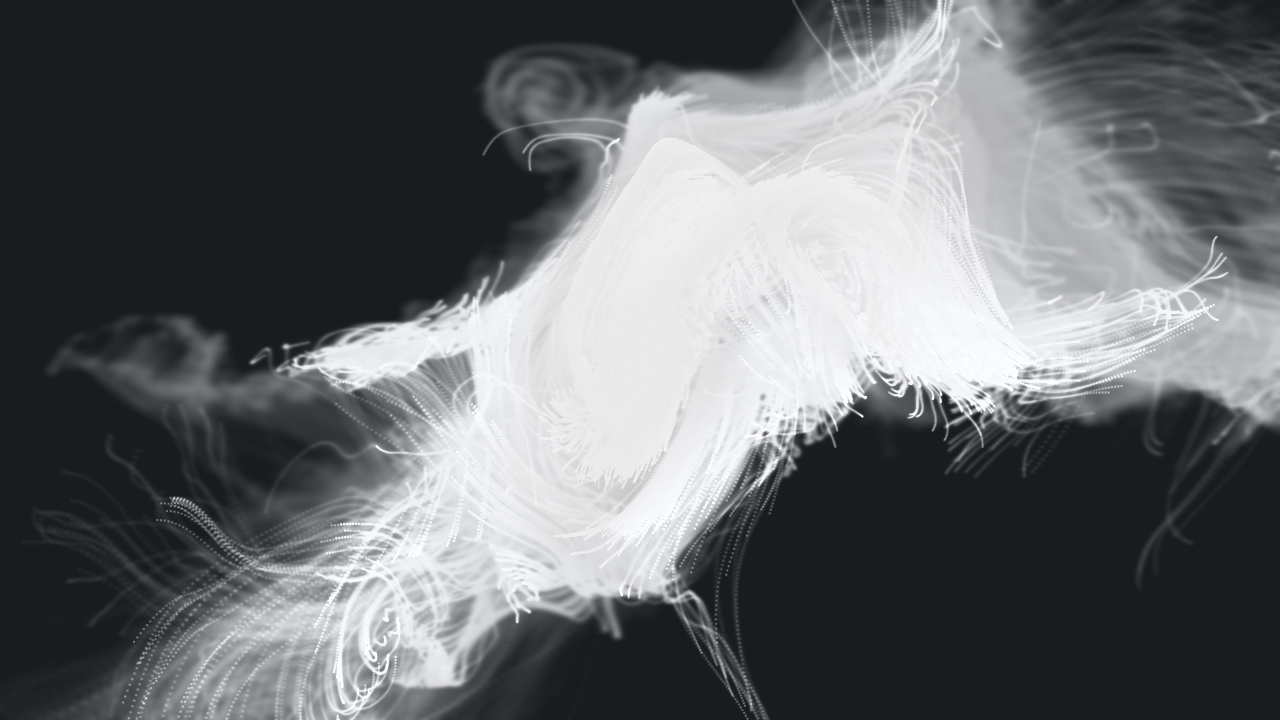
\includegraphics[width=\textwidth]{img/particle2.png}
	\caption[Particle system with feedback]
	{Particle system with feedback}
	\label{fig:label}
\end{figure}


\begin{figure}[H]
  \centering
  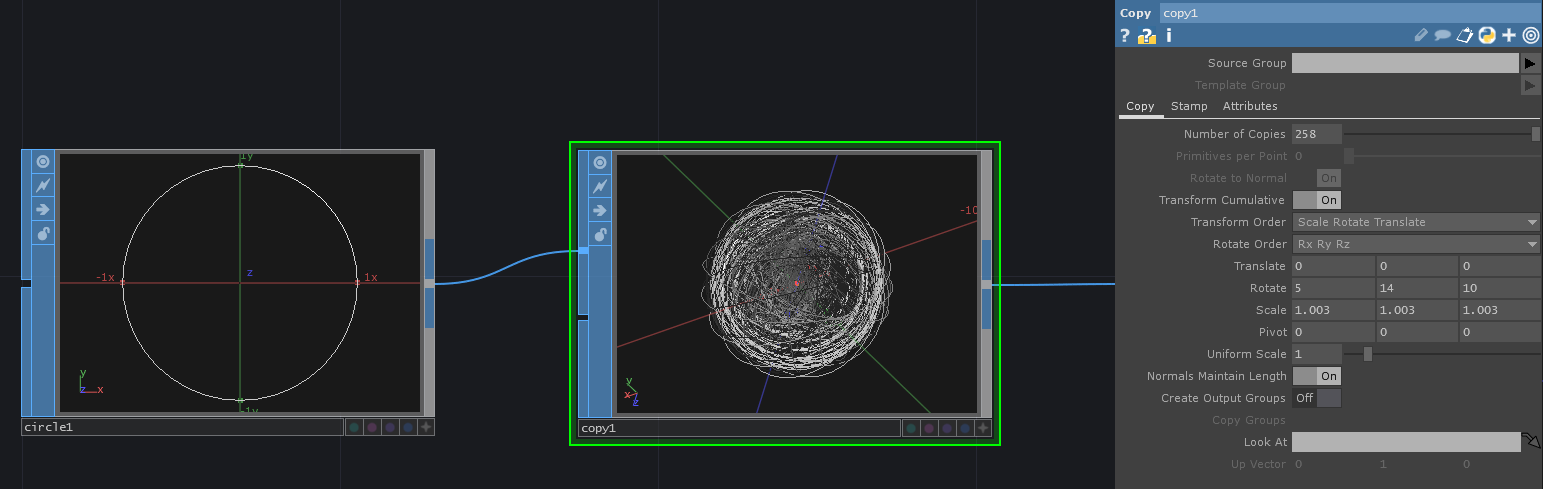
\includegraphics[width=\textwidth]{img/copySop.PNG}
  \caption[shortCaption]
  {CAPTION MISSING}
  \label{fig:label}
\end{figure}




\begin{figure}[H]
  \centering
  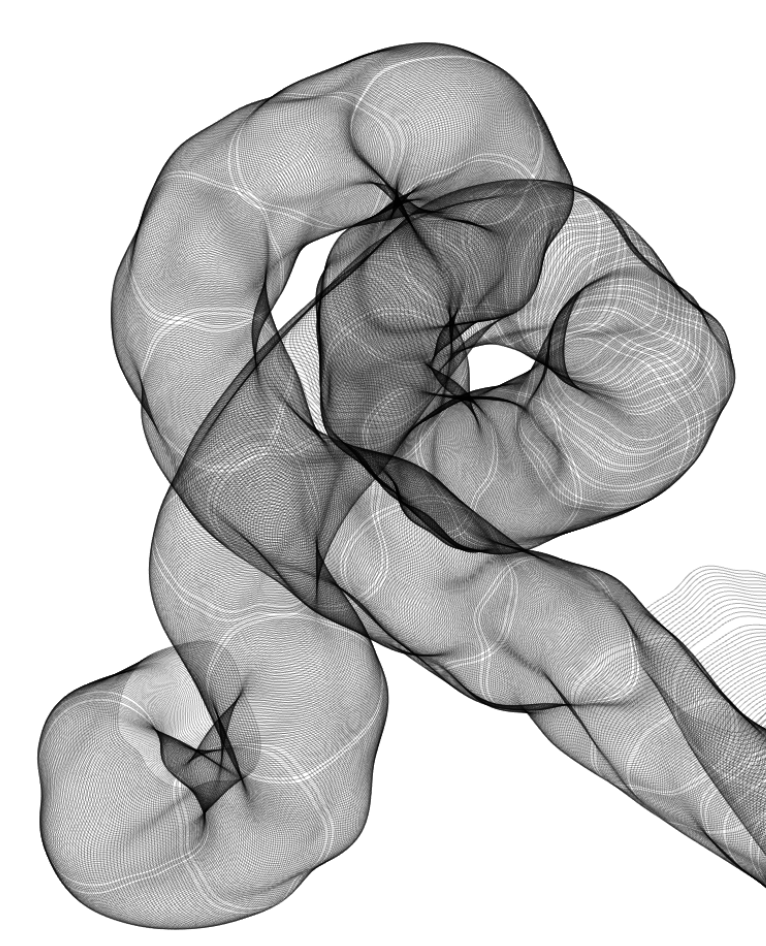
\includegraphics[width=10cm]{img/ggForms01.PNG}
  \caption[shortCaption]
  {CAPTION MISSING}
  \label{fig:label}
\end{figure}


\begin{figure}[H]
  \centering
  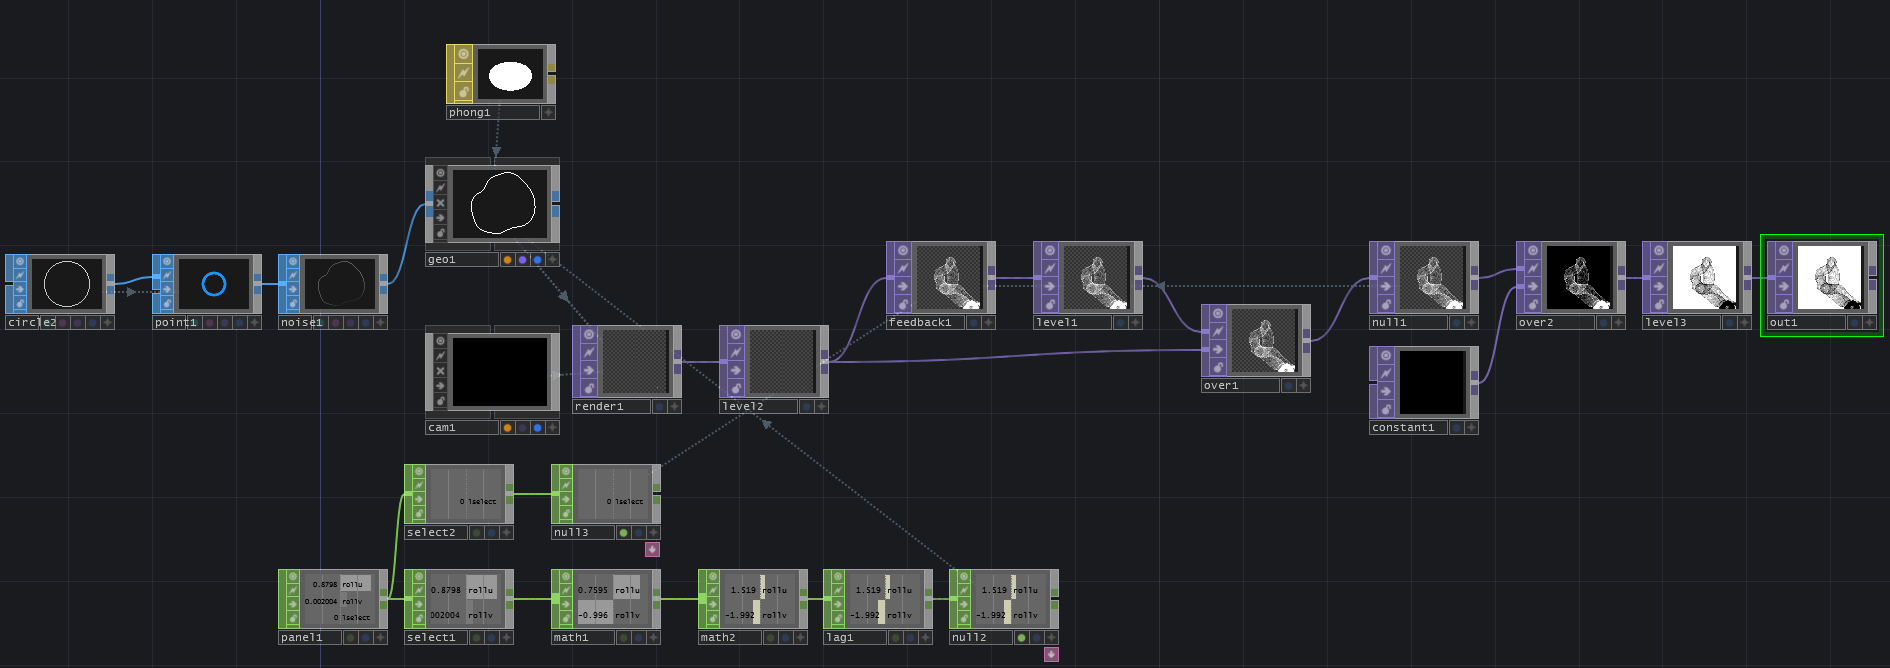
\includegraphics[width=\textwidth]{img/ggForms02.PNG}
  \caption[shortCaption]
  {CAPTION MISSING}
  \label{fig:label}
\end{figure}

\begin{figure}[H]
  \centering
  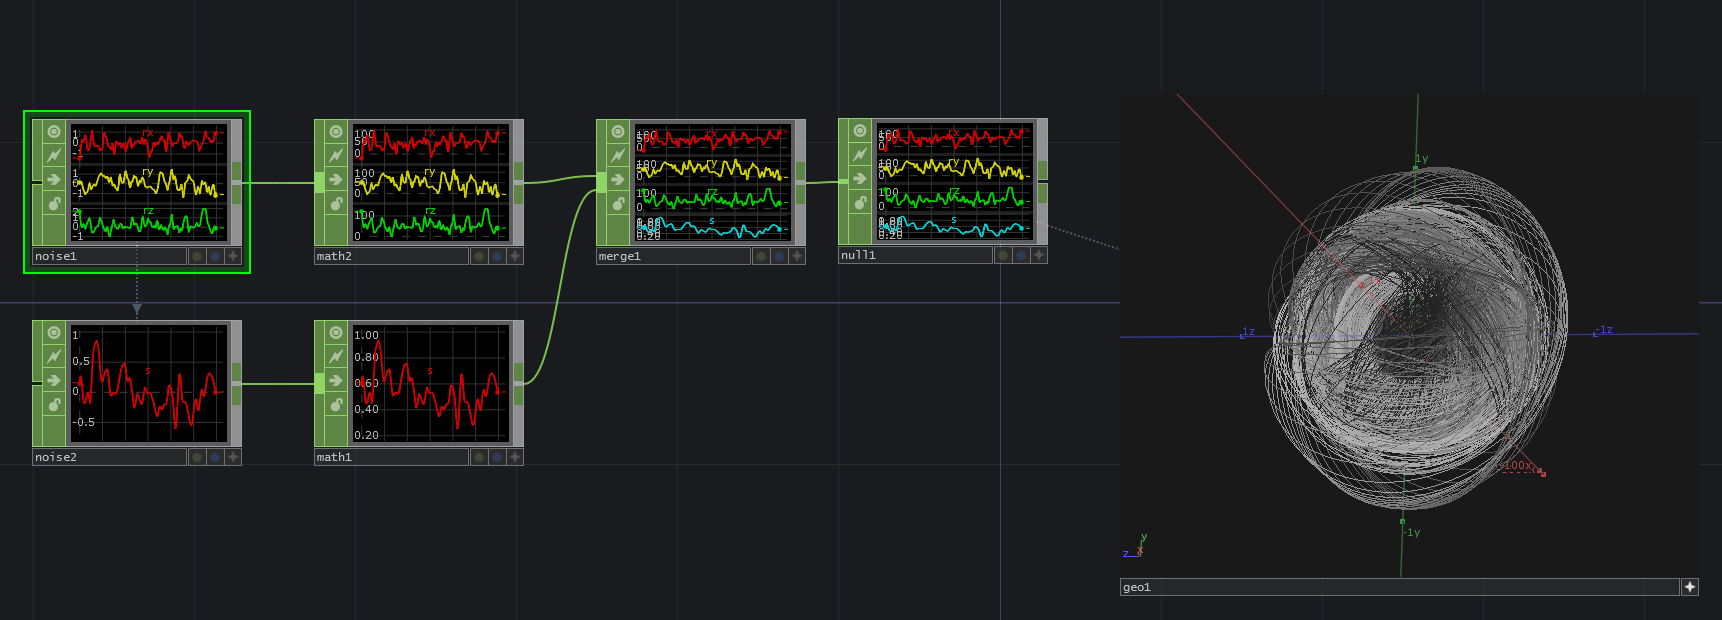
\includegraphics[width=\textwidth]{img/instancing1.PNG}
  \caption[shortCaption]
  {CAPTION MISSING}
  \label{fig:label}
\end{figure}

\begin{figure}[H]
  \centering
  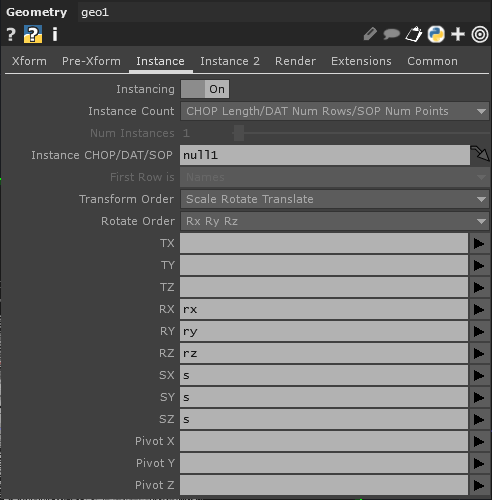
\includegraphics[width=8cm]{img/instancing2.PNG}
  \caption[shortCaption]
  {CAPTION MISSING}
  \label{fig:label}
\end{figure}

\begin{figure}[H]
  \centering
  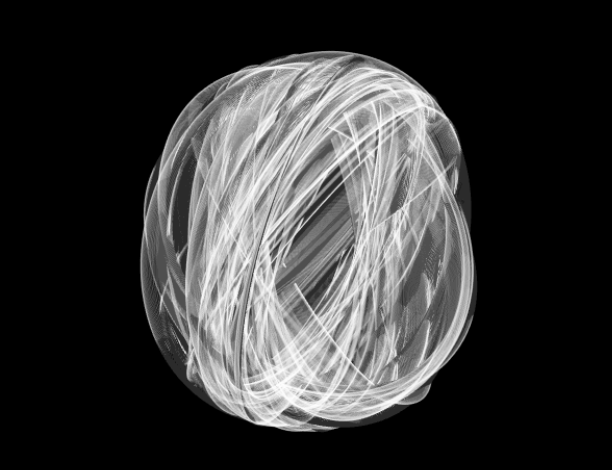
\includegraphics[width=10cm]{img/rings7200.PNG}
  \caption[shortCaption]
  {7200 circles in movement plus some material tweaking}
  \label{fig:label}
\end{figure}

\begin{figure}[H]
  \centering
  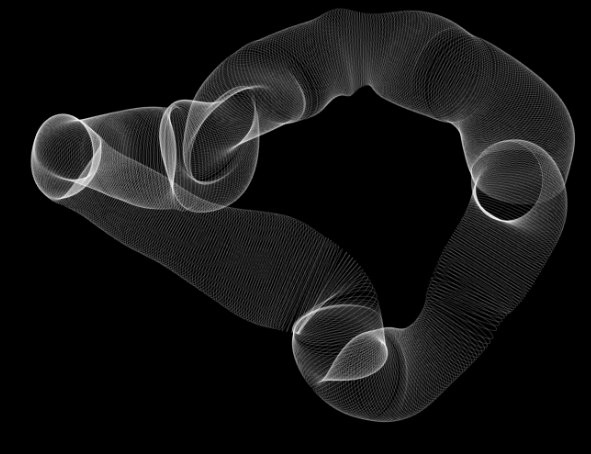
\includegraphics[width=\textwidth]{img/ggForms3d.PNG}
  \caption[shortCaption]
  {Three dimensional version of the generative design noise circle example}
  \label{fig:label}
\end{figure}



\begin{figure}[H]
	\centering
	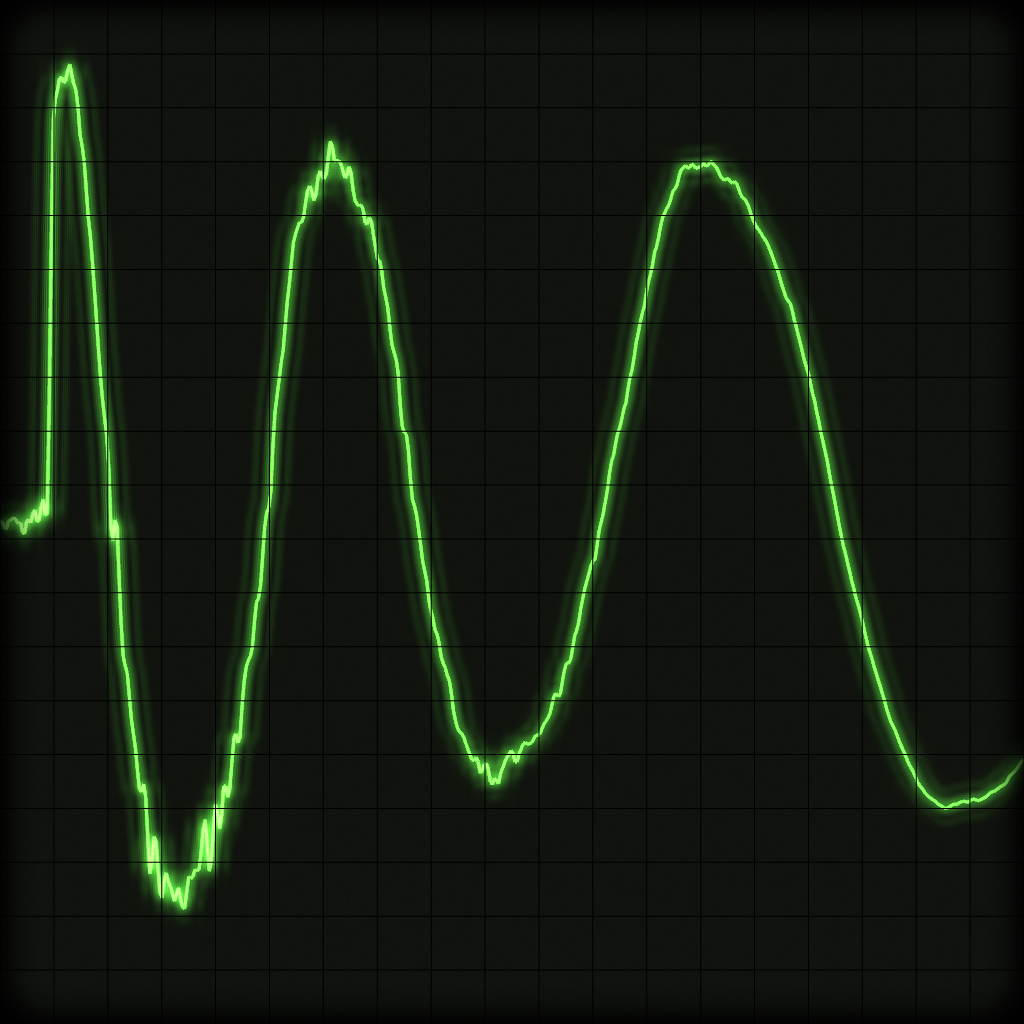
\includegraphics[width=10cm]{img/oscilloscope.png}
	\caption[shortCaption]
	{CAPTION MISSING}
	\label{fig:label}
\end{figure}


\begin{figure}[H]
  \centering
  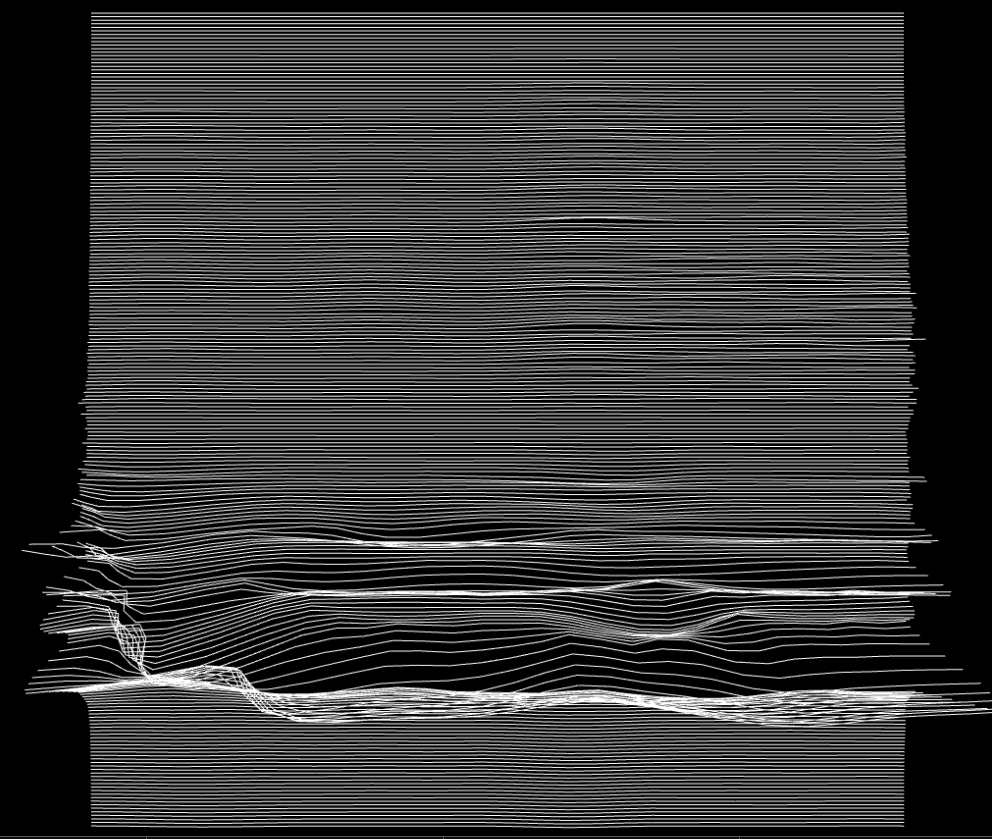
\includegraphics[width=\textwidth]{img/waterfall.PNG}
  \caption[shortCaption]
  {Waterfall plot of an audio spectrum}
  \label{fig:label}
\end{figure}


\begin{figure}[H]
	\centering
	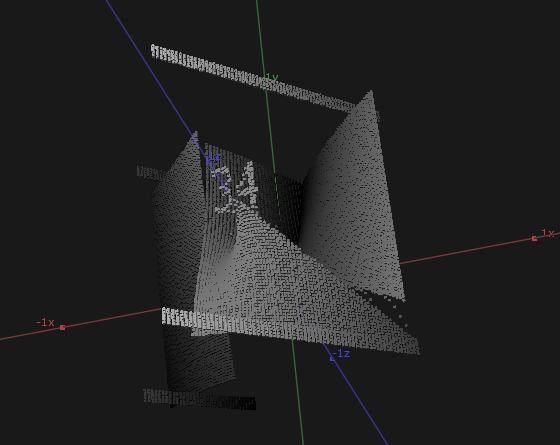
\includegraphics[width=\textwidth]{img/convert2Dto3D.PNG}
	\caption[shortCaption]
	{CAPTION MISSING}
	\label{fig:label}
\end{figure}



\begin{figure}[H]
	\centering
	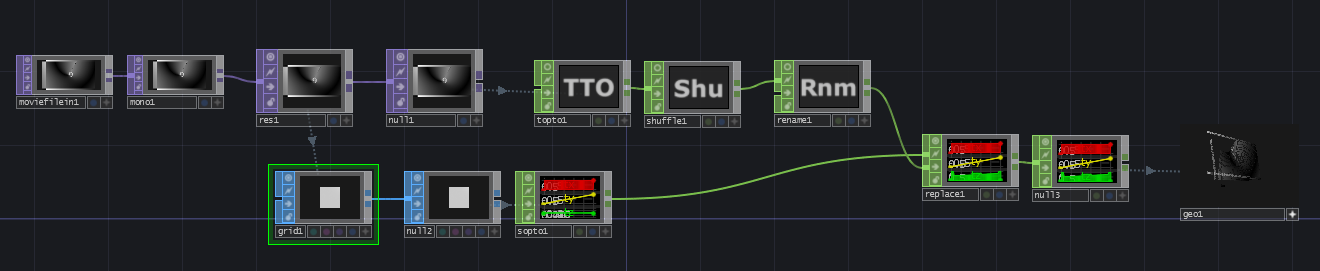
\includegraphics[width=\textwidth]{img/convert2Dto3D2.PNG}
	\caption[shortCaption]
	{CAPTION MISSING}
	\label{fig:label}
\end{figure}



\begin{figure}[H]
	\centering
	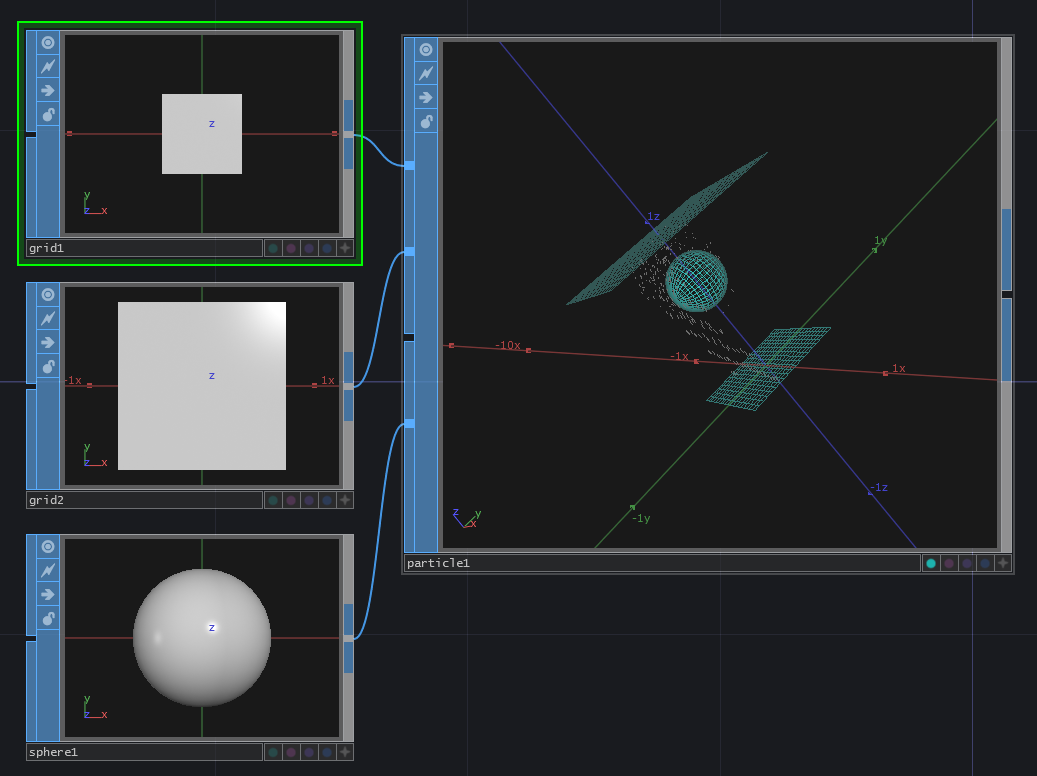
\includegraphics[width=\textwidth]{img/particles1.PNG}
	\caption[shortCaption]
	{CAPTION MISSING}
	\label{fig:label}
\end{figure}



\begin{figure}[H]
  \centering
  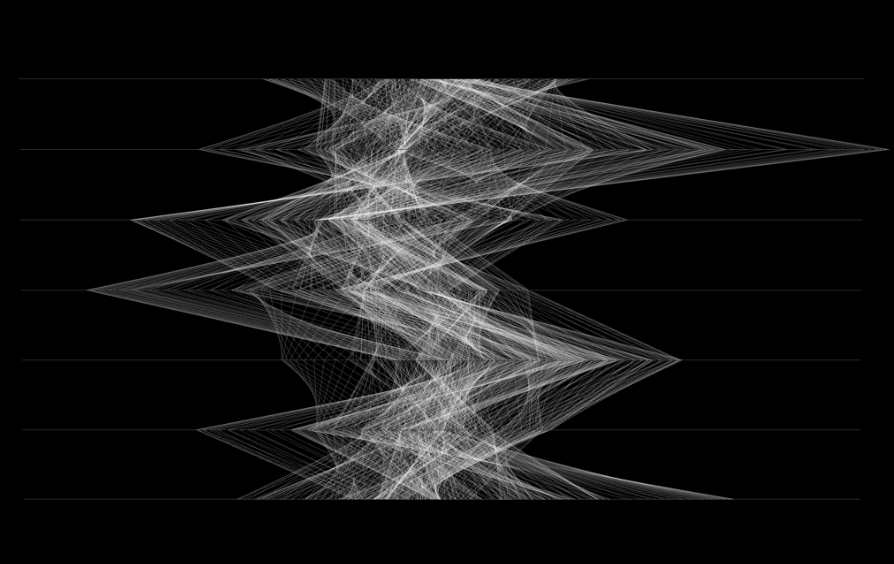
\includegraphics[width=\textwidth]{img/hyperDim.PNG}
  \caption[shortCaption]
  {'parallel Coordinates', a technique for hyperdimensional data visualization}
  \label{fig:label}
\end{figure}



%!TEX root = main.tex
%=================TD functions==================
\def\boldcommandlist{\@elt OP,\@elt OPs,}
\def\@elt#1,{%
 \expandafter\def\csname#1\endcsname{\textbf{#1}\xspace}
}
\boldcommandlist

\def\topColorList{\@elt TOP,\@elt TOPs,}
\def\@elt#1,{%
 \expandafter\def\csname#1\endcsname{\textcolor{TOP}{\textbf{#1}}\xspace}
}
\topColorList

\def\chopColorList{\@elt CHOP,\@elt CHOPs,}
\def\@elt#1,{%
 \expandafter\def\csname#1\endcsname{\textcolor{CHOP}{\textbf{#1}}\xspace}
}
\chopColorList

\def\sopColorList{\@elt SOP,\@elt SOPs,}
\def\@elt#1,{%
 \expandafter\def\csname#1\endcsname{\textcolor{SOP}{\textbf{#1}}\xspace}
}
\sopColorList

\def\datColorList{\@elt DAT,\@elt DATs,}
\def\@elt#1,{%
 \expandafter\def\csname#1\endcsname{\textcolor{DAT}{\textbf{#1}}\xspace}
}
\datColorList

\def\matColorList{\@elt MAT,\@elt MATs,}
\def\@elt#1,{%
 \expandafter\def\csname#1\endcsname{\textcolor{MAT}{\textbf{#1}}\xspace}
}
\matColorList


\def\compColorList{\@elt COMP,\@elt COMPs,}
\def\@elt#1,{%
 \expandafter\def\csname#1\endcsname{\textcolor{COMP}{\textbf{#1}}\xspace}
}
\compColorList

\def\redcommandlist{\@elt missingImage,}
\def\@elt#1,{%
 \expandafter\def\csname#1\endcsname{\textcolor{red}{\textbf{#1}}\xspace}
}
\redcommandlist

%===============================================

\chapter{Lecture 4}

\section{Notes}

\begin{itemize}
	\item more proc modeling
	\item parent shortcuts
	\item custom parameters
	\item modules
	\item structured work
	\item Cloning
	\item Replicator
	\item ui building
\end{itemize}

\section{Project Setup and Structure}

There are a lot of ways to set up a project for live performance. Different projects will require different structures and setups. Here, we will have a look at one suggestion. This suggestion is designed to fulfill the following criteria:
\begin{itemize}
	\item Being non-Linear and interactive
	\item Being somewhat tidy
	\item having multiple scenes
	\item having multiple FX
	\item each scene can be combined with each Effect
	\item Having a GUI
	\item each scene can react to audio without the need to duplicate the audio analysis
	\item versatile Output
	\item Minimize time for on-site configurations and adaptions
\end{itemize}


The project will be set up in a hierarchical way. In \texttt{root} we find a structure that looks like Figure \ref{fig:projectSchematic}.

	\begin{figure}[H]
	\centering


	% \resizebox{10cm}{!}{%
	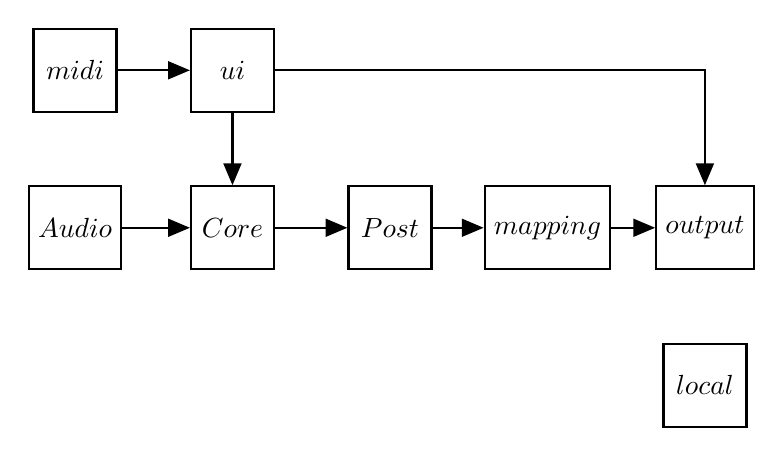
\begin{tikzpicture}[auto, thick, node distance=2.3cm, >=triangle 45]

	\draw node at (5,0) [block] (audio) {$Audio$};
	\draw node [block, right of=audio, node distance = 2cm] (core) {$Core$};
	\draw node [block, right of=core, node distance = 2cm] (post) {$Post$};
	\draw node [block, right of=post, node distance = 2cm] (mapping) {$mapping$};
	\draw node [block, right of=mapping, node distance = 2cm] (output) {$output$};
	\draw node [block, below of=output, node distance = 2cm] (local) {$local$};
	\draw node [block, above of=audio, node distance = 2cm] (hid) {$midi$};
	\draw node [block, above of=core, node distance = 2cm] (ui) {$ui$};

  \draw[->] (hid) -- node {}(ui);
  \draw[->] (ui) -- node {}(core);
  \draw[->] (audio) -- node {}(core);
  \draw[->] (core) -- node {}(post);
  \draw[->] (post) -- node {}(mapping);
  \draw[->] (ui) -| node {}(output);
    \draw[->] (mapping) -- node {}(output);

  \end{tikzpicture}
  \caption{Schematic view of our project}
  \label{fig:projectSchematic}
\end{figure}

In practice, this might look like in Figure \ref{fig:structPraxis}.
\begin{figure}[H]
	\centering
	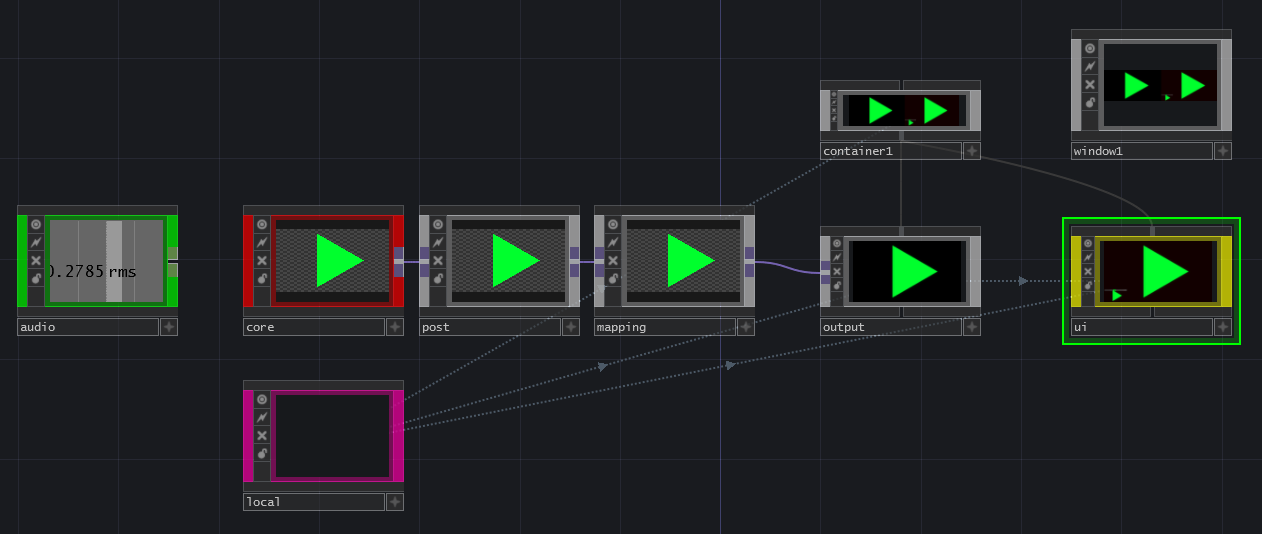
\includegraphics[width=\textwidth]{img/structure1.PNG}
	\caption[shortCaption]
	{Root level of our Project, inside \texttt{/project1/}}
	\label{fig:structPraxis}
\end{figure}

Notice that some arrows exist in the schematic but don't have corresponding patch cords in Figure \ref{fig:structPraxis}. This is because the information is flowing via references and/or Select \OPs.

Let's now have a look at what happens in each of these \COMPs.

\paragraph*{Midi}
We could also name this 'HID'(Human Interface devices). This could manage OSC\footnote{Open Sound control, a very common protocol for inter device communication typically running on top of the UDP protocol}. Typically some form of hardware device is used to control elements on the UI which then control the actual parameters.
\paragraph*{UI}
The UI Component is typically a Container \COMP. It holds the Graphical User Interface we see during our Show. It contains Sliders and other controls, previews of currently unused scenes and shows us our actual output in case we don't see our projection. It should also show us some information about audio input levels (This is not shown in figure \ref{fig:projectSchematic}).
Also it is used by the output, since we typically create one window spanning over all our monitors.\\
The UI can instantiate other UIs and can hold stored data.
\paragraph*{Audio}
Here we find our audio input (Audio Device In \CHOP) and all the audio analysis. The analyzed values (e.g. the current RMS) is then used by scenes in \texttt{core}.
\paragraph*{Core}
Here we actually create our different scenes and effects.
A very typical setup inside \texttt{core} could look like Figure \ref{fig:coreSchematic}. This is only one possibly topology of our image generation. We could also create our show using just one versatile algorithm with many parameters and possibly preset store/load facilities or we could go for a more interconnected matrix-like layout.


\begin{figure}[H]
	\centering

	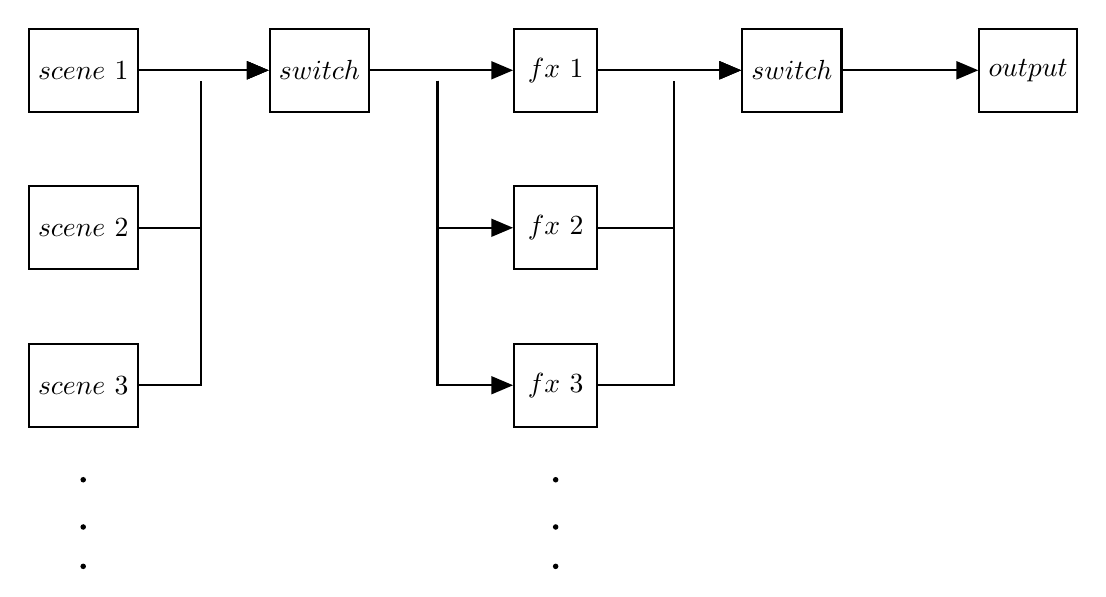
\begin{tikzpicture}[auto, thick, node distance=2.3cm, >=triangle 45]

	\draw node at (5,0) [block] (scene1) {$scene\ 1$};
	\draw node [block, below of=scene1, node distance = 2cm] (scene2) {$scene\ 2$};
	\draw node [block, below of=scene2, node distance = 2cm] (scene3) {$scene\ 3$};

	\draw node [block, right of=scene1, node distance = 3cm] (switch1) {$switch$};
	\draw node [block, right of=switch1, node distance = 3cm] (fx1) {$fx\ 1$};
	\draw node [block, below of=fx1, node distance = 2cm] (fx2) {$fx\ 2$};
	\draw node [block, below of=fx2, node distance = 2cm] (fx3) {$fx\ 3$};

	\draw node [block, right of=fx1, node distance = 3cm] (switch2) {$switch$};

	\draw node [block, right of=switch2, node distance = 3cm] (output) {$output$};

	\foreach \point in {(5,-5.2),(5,-5.8),(5,-6.3)}{% points
    \fill \point circle (1pt);
}
\foreach \point in {(11,-5.2),(11,-5.8),(11,-6.3)}{% points
    \fill \point circle (1pt);
}



	\draw  node [right of=scene1, node distance = 1.5cm] (bp){};
	\draw  node [right of=switch1, node distance = 1.5cm] (bp2){};
	\draw  node [right of=fx1, node distance = 1.5cm] (bp3){};

	\draw[->] (scene1.east) -- node {}(switch1);
	\draw[->] (scene2.east) -| node{}(bp) -- node {}(switch1);
	\draw[->] (scene3.east) -| node{}(bp) -- node {}(switch1);

	\draw[->] (switch1) -- node {}(fx1);
	\draw[->] (switch1) -- node{}(bp2) |- node {}(fx2);
	\draw[->] (switch1) -- node{}(bp2) |- node {}(fx3);

	\draw[->] (fx1) -- node {}(switch2);
	\draw[->] (fx2) -| node{}(bp3) -- node {}(switch2);
	\draw[->] (fx3) -| node{}(bp3) -- node {}(switch2);

	\draw[->] (switch2) -- node {}(output);

  \end{tikzpicture}
  \caption{Schematic view of \texttt{core}}
  \label{fig:coreSchematic}
\end{figure}

In reality, this could look like Figure \ref{fig:insideCore}.

\begin{figure}[H]
	\centering
	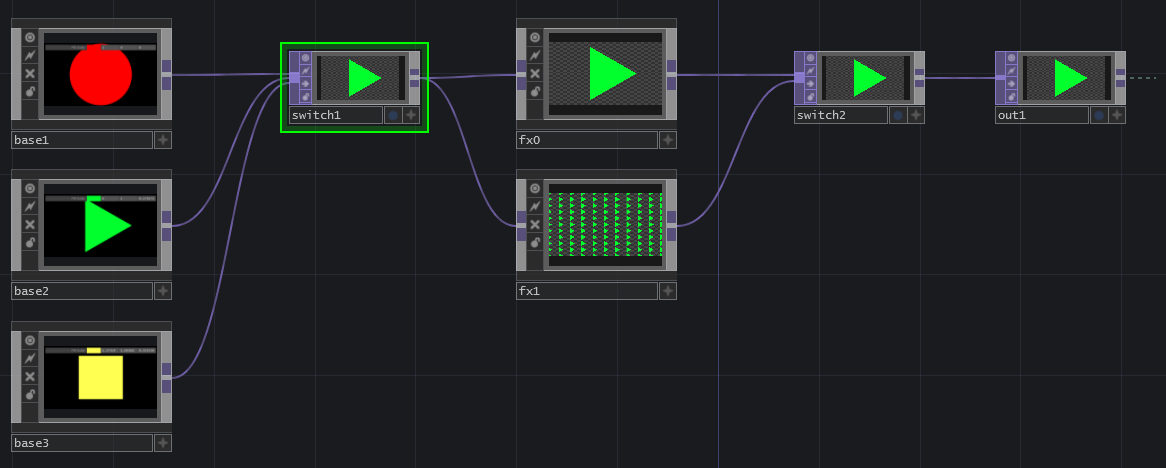
\includegraphics[width=\textwidth]{img/structure2.PNG}
	\caption[shortCaption]
	{inside \texttt{/project1/core}}
	\label{fig:insideCore}
\end{figure}


\paragraph*{Post}
Oftentimes we need some simple post fx such as contrast and color correction feature for adjustment on-site.
\paragraph*{Mapping}
Here we might do our mapping for example using \textbf{Cam Schnappr} or \textbf{Kantan Mapper}. Both of these tools can be found in TouchDesigner's Palette.
\paragraph*{Output}
Our output can be a Window \COMP inside of \texttt{project1}. It should contain both our UI and the image we want to send to our projector(s).
\paragraph*{Local}
The \texttt{local} \COMP is a special \COMP. It simply is a Base \COMP that we renamed to \texttt{local}. This in turn makes TouchDesigner look in there for modules and variables. We will have a look at this at a later point, but to put it simply: It allows us to store states, paths and other variables that make our network more manageable.



\section{Designing a self-contained Component, our first Scene}
Let's have a look at an example scene first:

\begin{figure}[H]
	\centering
	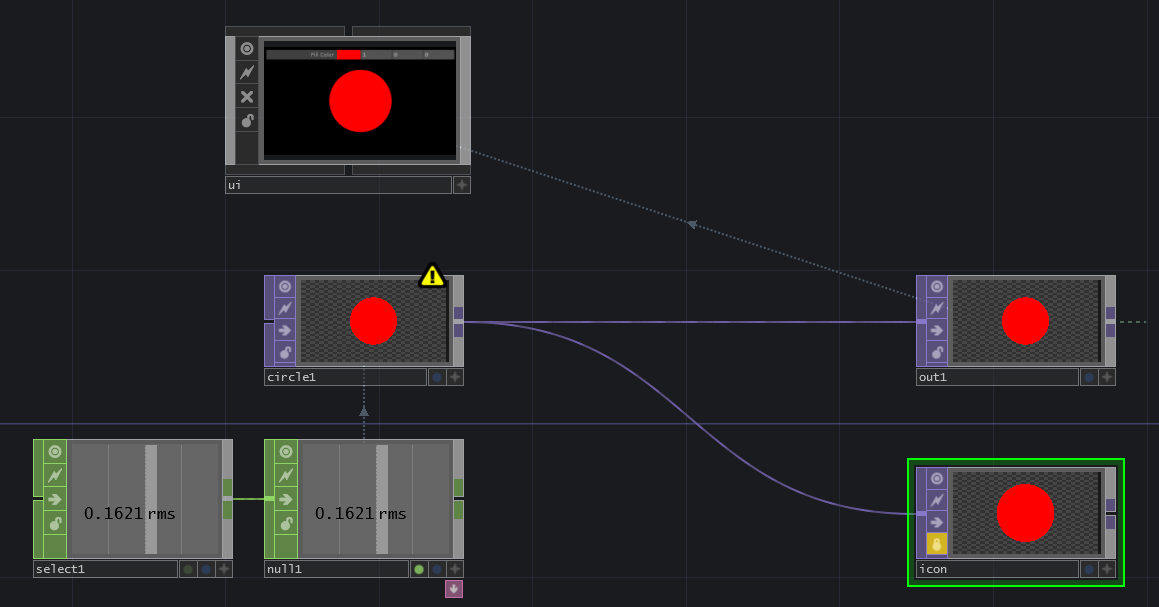
\includegraphics[width=\textwidth]{img/exampleScene.PNG}
	\caption[example scene]
	{example scene, \texttt{/project1/core/scene0}}
	\label{fig:label}
\end{figure}

What we have is some super simplistic imige generator, that is controlled via the RMS of the audio. It's output is sent to the \COMP's output. Also its output was cached at some point into a Null \TOP with the Lock Flag enabled to save the image. The Null \TOP is renamed to \texttt{icon}. This is a convention to later fetch an unanimated preview of what the scene looks like.\\
Also we have a simple GUI in form of a Component \COMP.\\
So let's now see why we chose to layout our exmaple scene this way and what concepts were used here and why.\\

Ideally our scenes are self contained in a sense that we can drag and drop them in any network, they work instantly and we never have to look inside. How can we achieve this? Basically via
\begin{itemize}
	\item \link{https://docs.derivative.ca/index.php?title=Custom\_parameters}{Custom Parameters}
	\item a decent GUI
	\item Sticking to certain standards
	\item enough interconnectivity
	\item Testing. Make sure there are no errors. Because there are errors.
\end{itemize}

We will now have a look at how to build a GUI and how to expose parameters.
An excellent video about how to build components can be found \link{https://www.youtube.com/watch?v=3mgn5SJg1oI}{here}
\subsection{Custom Parameters}
\index{customize component}
\index{custom parameters}
The Custom Parameters feature allows us to add parameters to a Component. We can just right-click on a Component an choose \texttt{Customize Component...} to arrive at the window shown in Figure \ref{fig:customizeComponent}.

\begin{figure}[H]
	\centering
	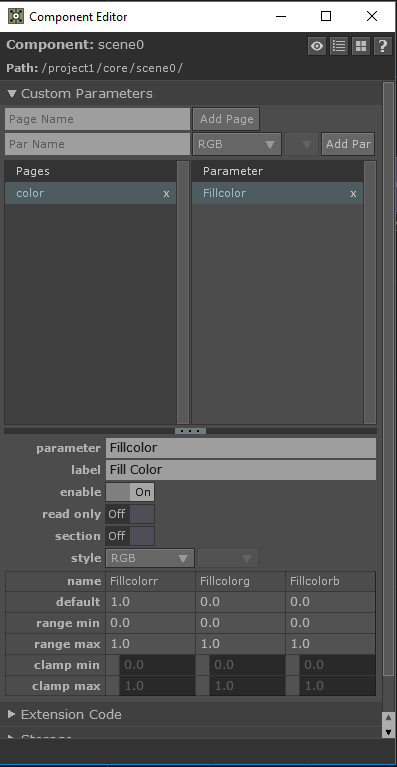
\includegraphics[width=8cm]{img/customizeComponent.PNG}
	\caption[customize component]
	{The Component Editor}
	\label{fig:customizeComponent}
\end{figure}

Here we can add pages and parameters to our component's parameter dialog.\\
Often we will just need to control a parameter of one of our \OPs inside the \COMP directly. We would need to look at the parameter, find the correct type for our custom parameter, and link it to the parameter inside via an expression or CHOP exporting. But there is a nice trick:
We can open the Component Editor, go inside our Component and drag the parameter we want to control to the Parameter list in the Component Editor. This will create a new Parameter with the same name, type and ranges as the original parameter. Also there appears a small pop-up, asking us if we want to automatically create a reference, so the two are linked.

\subsection{Simple GUI}

TouchDesigner is really good for GUI building.
\begin{figure}[H]
	\centering
	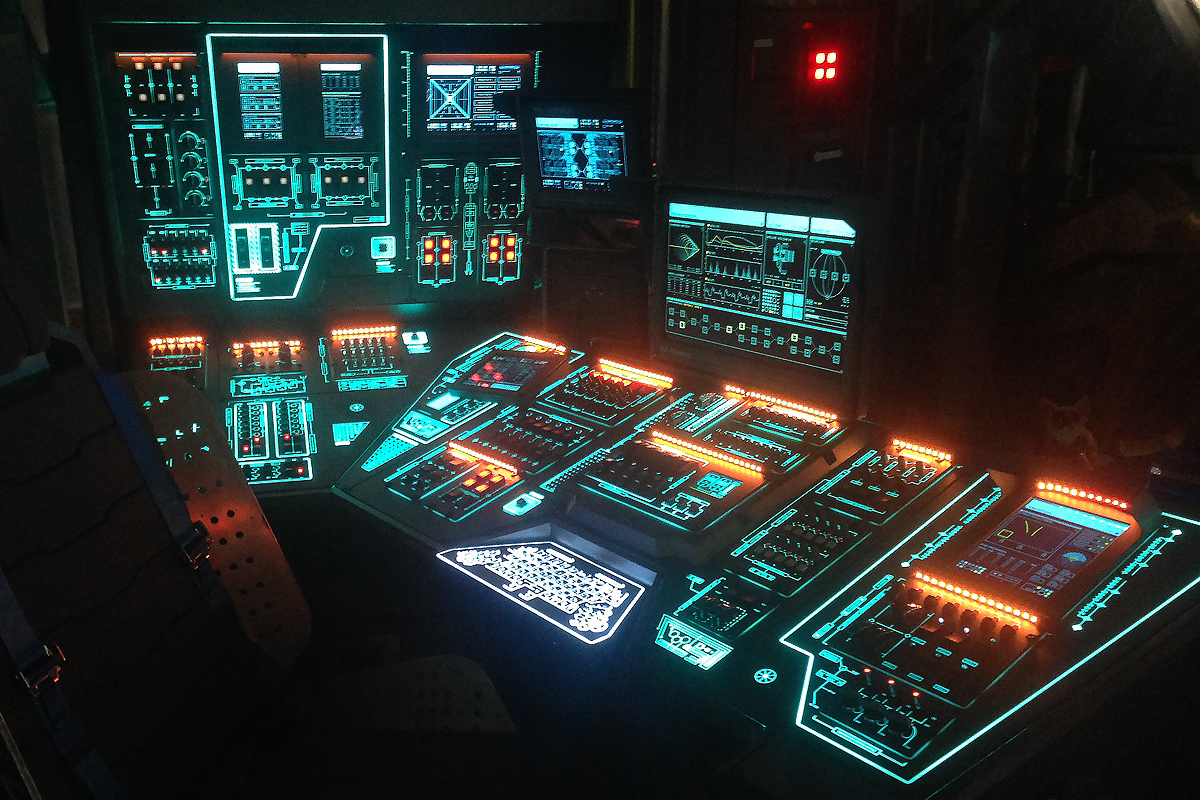
\includegraphics[width=\textwidth]{img/alien.jpg}
	\caption[shortCaption]
	{Image taken from \link{http://derivative.ca/events/2017/AlienCovenant/}{here}. GUIs built in TouchDesigner for the motion picture Alien Covenant}
	\label{fig:label}
\end{figure}


But before getting to complicated, let's look at how we can get the most simplistic GUI going. For our scenes, it would be great if we had a GUI that showed the output of our scene and the important parameters. GUIs are built using one or multiple Container \COMPs.\\
The Container \COMP allows us to align children elements in an orderly hierarchical manner and it generates events and data for mouse interaction such as mouse rollover or click events. \\
Another very handy \COMP is the Parameter \COMP. We can just point it to a parameter of a chosen OP and it displays it.\\
So, to make our example scene display a very simple GUI, we do the following:

\begin{enumerate}
	\item create a Container \COMP
	\item rename it to 'ui'
	\item point its \texttt{background TOP} parameter to out Out \TOP
	\item inside the Container \COMP, create a Parameter \COMP.
	\item adjust the Parameter \COMP to point to important parameters.
	\item in the \texttt{OP Viewer} parameter of our \texttt{scene0} Base \COMP, write \texttt{./ui}, so the scene displays its ui
\end{enumerate}





\subsection{Connections without Patch Cords, the Select OPs}

\begin{figure}[H]
	\centering
	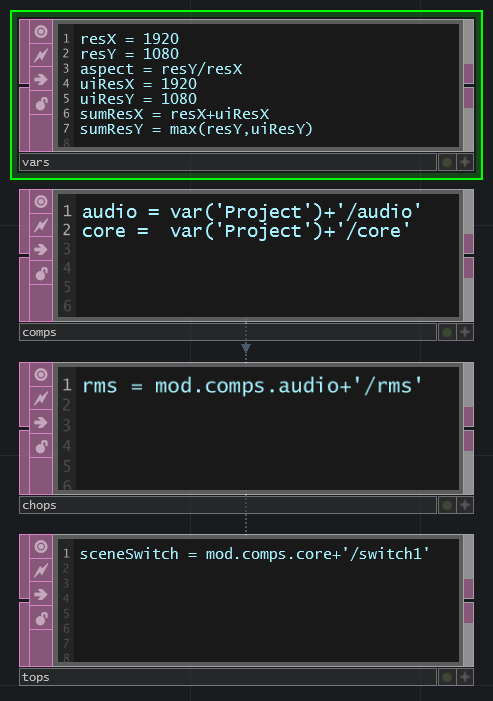
\includegraphics[width=8cm]{img/localModules.PNG}
	\caption[shortCaption]
	{CAPTION MISSING}
	\label{fig:label}
\end{figure}




\subsection{Configuring TD after Install} % (fold)
\label{sub:config}
There are not a lot of things that have to be configured after a fresh install of TD. One of the things that are highly recommended to be adjusted is the text editor\index{text editor}. Sometimes, we write actual text-code inside TouchDesigner, be it \textbf{python}, \textbf{GLSL}, \textbf{TScript}, or another language. We can write this code inside TD itself, but we can also use an external text editor, such as Sublime Text or Notepad+, which provides syntax highlighting, auto-completion and more.\\
In order to conveniently use such an external editor, we just need to go to TD's preferences and specify the path to the external editor.

% to set an \textbf{Environment Variable}. In Windows, there is an application for setting those, the easiest way to access this application is to just search it in the start menu, it's called \textit{Umgebungsvariablen Für dieses Konto bearbeiten} or \textit{Environment Variables}.\\
% Here, a variable called \verb|TOUCH_EDITOR| should be created and it's value should be set to the path to your favorite text editor.\\
After that, anytime we right-click on a \DAT and choose \textit{Edit contents} or press \keystroke{ctrl}+\keystroke{e}, our text editor opens, we can edit the file, save it and will have edited that \DAT.



\subsection{Scripting} % (fold)
\label{sub:scripting}
important helper functions:\\
\begin{lstlisting}
	dir(object) #get attributes of the object
	help(object) #call help on object
\end{lstlisting}

\subsubsection{Referencing \OPs} % (fold)
\label{ssub:referencing}
\OPs and their contents can be referenced in an absolute or relative way. Also, it makes sense to save paths inside variable\index{variable}, as we will see in \ref{ssub:Modules}. to reference a Null \CHOP at \verb|/project1/null1| for example, we can use the expression:
\begin{lstlisting}
	op('/project1/null1')
\end{lstlisting}
We can access the first channel in that Null \CHOP just by issuing \verb|op('/project1/null1')[0]|. Also, a \CHOP's channels may be accessed by their name, so if we had a \CHOP with a channel named \verb|tx| at the same location, we can use \verb|op('/project1/null1')['tx']|. Both of these expressions are useful for animating parameters, and are an alternative to \textbf{CHOP exporting}(see \ref{sub:CHOPs}).

\begin{framed}
	What should I use, \CHOP exporting or python references?
	Python expressions and references tend to be cleaner and more readable.
	\CHOP exporting is faster performance-wise. The team at derivative is constantly working to make python expressions compile to native C code in the backround so simple expresions and references are basically already as fast as \CHOP exporting. \\
	So, if in a certain project, performance is a very critical issue, one should still stick to \CHOP exporting. Otherwise, python expressions are preferable due to readability and overall handyness.
\end{framed}

\subsubsection{Variables} % (fold)
\label{ssub:variables}

In TouchDesigner, there are a number of variable types \footnote{\href{http://www.derivative.ca/wiki088/index.php?title=Variables}{Variables on the TouchDesigner Wiki}}. Within scripts, variables may be defined in a standard pythonic way, such as \verb|a = 5|. For variables that may be accessed throughout a network, \textbf{component variables} are the most useful ones, although
there are a couple of options to get a variable-like behavior\footnote{Other options, that might be more useful depending on the situation are: Referencing a
Null \CHOP, extensions, the storage system, modules containing variables and more}, without defining an actual variable.\\
Variables in TD should not be used for processes that require them to be written very often, such as driving an animation at 60 FPS with a variable. A (time sliced) \CHOP channel makes more sense in such situations. Think of variables rather for purposes of storing application resolution, setting and getting the state of state machines, or similar \glqq{}semi-static\grqq{} values.\\

Component variables in TD are bound to a \COMP. They can be bound to the \textbf{root Component}, but may live in any component. There are many ways to get the value of a variable, as well as setting it. In order to create a variable called \verb|varName|
with the value \verb|5| in the component \verb|/project1| we can execute the command:
\begin{lstlisting}
	op('/project1').setVar('varName', 5)
\end{lstlisting}

This will create a Base \COMP: \verb|/project1/local|. The \verb|local| \COMP is a special \COMP that is automatically referenced in certain situations, such as retrieving a variable or module. We could have created a Base \COMP and renamed it to \verb|local| manually too. Inside this \COMP, our variables are stored via \DATs.\\

 \missingImage \\

For defining variables that can be retrieved everywhere in a network, we typically define a component Variable that is attached to the root component (at \verb|/|). In order to do so, we can execute the command:
\begin{lstlisting}
	root.setVar('varName', 5)
\end{lstlisting}
This will store our new variable inside \verb|/local|. We can now get the value of \verb|varName| by evaluating
\begin{lstlisting}
	var('varName')
\end{lstlisting}
in a parameter or by using an Evaluate \DAT for example, but also simply in the \textbf{Text Port}.


We can override Variables inside specific \COMPs. Let's assume we made a complex network, and we use two root Component variables to set the resolution for all \TOPs in the network. This is good practice, since it makes it easy to change the resolution quickly and globally. But maybe we have some subprocess that is also quite complex and which needs a different resolution. We could make new variables. But what if we could just override the global ones inside just this subprocess? Well, we can, we just need to redefine the variables inside that specific \COMP.\\

Assume our complex subprocess is a base \COMP at \verb|/project1/sub|. We can just define:
\begin{lstlisting}
	root.setVar('resXY', [1280, 720])
	op('/project1/sub').setVar('resXY', [256, 256])
\end{lstlisting}
This way, everywhere in our network, \verb|resXY| will evaluate to the list \verb|[1280, 720]|, but everywhere inside \verb|/project1/sub| it will evaluate to \verb|[256, 256]|.

% subsubsection component_variables (end)
\subsubsection{Modules} % (fold)
\label{ssub:Modules}
\index{Module}Modules are a way to organize variables, functions, classes. Any Text \DAT can hold a module.
let's assume we made a Text \DAT at \verb|/project1/myTools|. In there, we wrote:
\begin{lstlisting}
	x = 5
	def multiplyByTwo(inp):
		return inp*2.
\end{lstlisting}
\testThis


We can now use this Text \DAT as a module. In order to do so, we have couple of options. One would be to use it in another script inside another Text \DAT. For example:
\begin{lstlisting}
	import myTools
	print (myTools.multiplyByTwo(5))
\end{lstlisting}

Another and maybe more common way would be to use it in a parameter, by the MOD (module on demand) class. If our module is inside the search Path (so in the same \COMP for example, or, as we see in a moment, inside \verb|local|) we can use the expression:
\begin{lstlisting}
	mod.myTools.multiplyByTwo(5)
\end{lstlisting}

For information on how to reference a module, and for information about how to import it as efficiently as possible, look \link{http://www.derivative.ca/wiki088/index.php?title=MOD\_Class}{here}


%!TEX root = main.tex

%=================TD functions==================
\def\boldcommandlist{\@elt OP,\@elt OPs,}
\def\@elt#1,{%
 \expandafter\def\csname#1\endcsname{\textbf{#1}\xspace}
}
\boldcommandlist

\def\topColorList{\@elt TOP,\@elt TOPs,}
\def\@elt#1,{%
 \expandafter\def\csname#1\endcsname{\textcolor{TOP}{\textbf{#1}}\xspace}
}
\topColorList

\def\chopColorList{\@elt CHOP,\@elt CHOPs,}
\def\@elt#1,{%
 \expandafter\def\csname#1\endcsname{\textcolor{CHOP}{\textbf{#1}}\xspace}
}
\chopColorList

\def\sopColorList{\@elt SOP,\@elt SOPs,}
\def\@elt#1,{%
 \expandafter\def\csname#1\endcsname{\textcolor{SOP}{\textbf{#1}}\xspace}
}
\sopColorList

\def\datColorList{\@elt DAT,\@elt DATs,}
\def\@elt#1,{%
 \expandafter\def\csname#1\endcsname{\textcolor{DAT}{\textbf{#1}}\xspace}
}
\datColorList

\def\matColorList{\@elt MAT,\@elt MATs,}
\def\@elt#1,{%
 \expandafter\def\csname#1\endcsname{\textcolor{MAT}{\textbf{#1}}\xspace}
}
\matColorList


\def\compColorList{\@elt COMP,\@elt COMPs,}
\def\@elt#1,{%
 \expandafter\def\csname#1\endcsname{\textcolor{COMP}{\textbf{#1}}\xspace}
}
\compColorList

\def\redcommandlist{\@elt missingImage,}
\def\@elt#1,{%
 \expandafter\def\csname#1\endcsname{\textcolor{red}{\textbf{#1}}\xspace}
}
\redcommandlist

%===============================================

\chapter{Lecture 5}

\section*{Notes}

\section*{Contents}

\subsection*{Pitch Visualization (Bach Piece)} % (fold)
\subsection*{Communication with Max/MSP} % (fold)
\subsection*{Projection Mapping} % (fold)
\subsection*{GLSL}
\subsection*{Procedural Modeling} % (fold)
https://www.shadertoy.com/view/MdfBRX

\label{sub:procedural_modeling}

\begin{itemize}
	\item group SOP
	\item latice SOP
	\item magnet/force/metaball SOP
	\item Texture SOP
	\item Model SOP
\end{itemize}

\section{Projection Mapping}
\link{https://docs.derivative.ca/index.php?title=Projection\_mapping}{Projection Mapping}

\subsection{2D Mapping}
There are a couple of \TOPs that enable us to do simple mapping tasks:
\begin{itemize}
	\item \refTOP{Crop}
	\item \refTOP{Corner\_Pin}
	\item \refTOP{Transform}
	\item \refTOP{Displace}
\end{itemize}
So if we jsut need some slight adjustment of our output we can come up with our own mapping tool. This keeps our network simple and is a good choice if we need nothing fancy.\\
For more complex 2D mapping scenarios TouchDesiger comes with some pretty advanced tools that helps us to properly map one or multiple textures to the physical environment.

\subsubsection{Stoner}
The \link{https://docs.derivative.ca/index.php?title=Palette:Stoner}{Stoner} \COMP can be found in the Palette.

\begin{figure}[H]
	\centering
	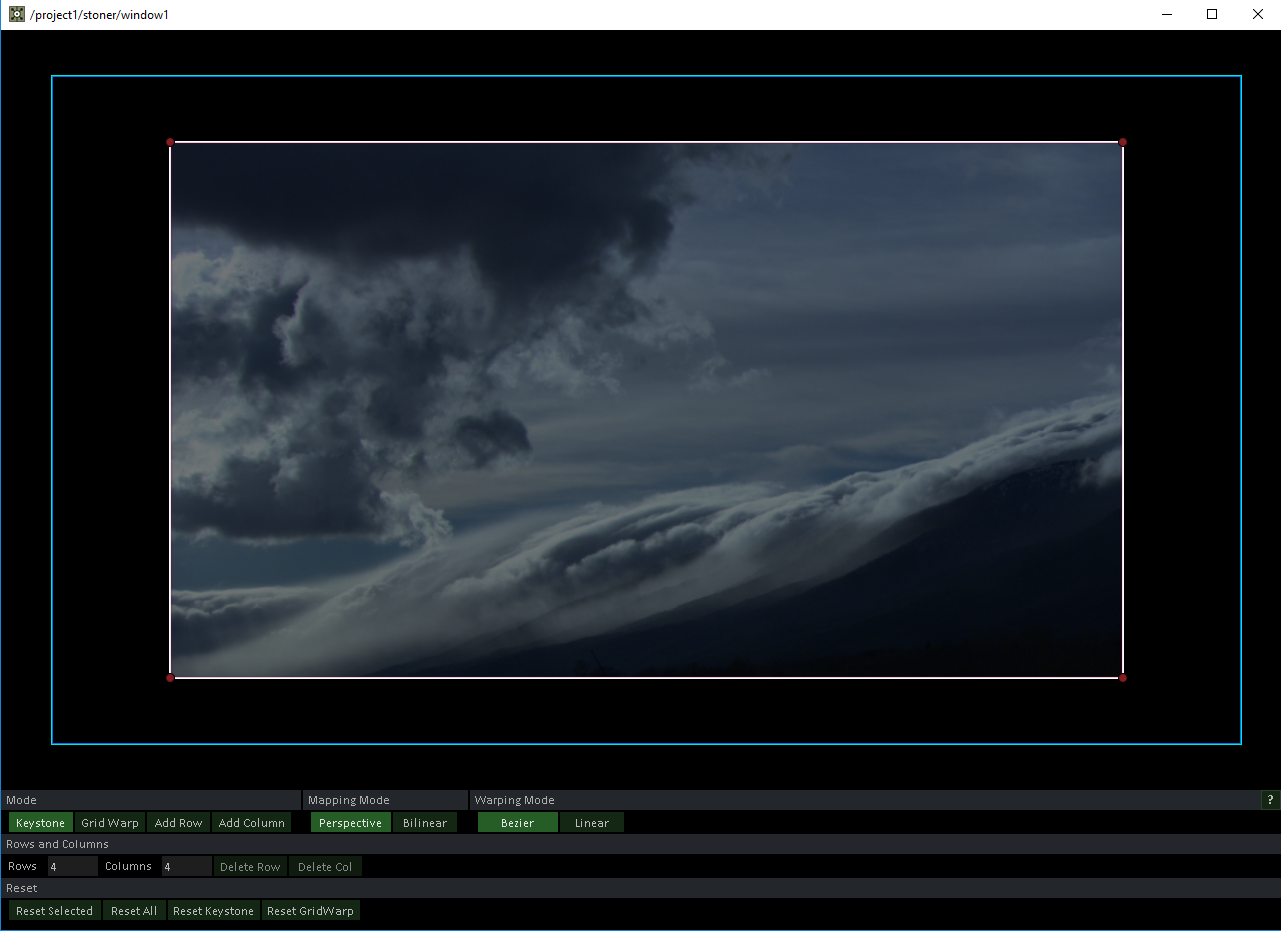
\includegraphics[width=\textwidth]{img/stoner.PNG}
	\caption[shortCaption]
	{CAPTION MISSING}
	\label{fig:label}
\end{figure}

\subsubsection{Kantan Mapper}
The \link{https://docs.derivative.ca/index.php?title=Palette:kantanMapper}{Kantan Mapper} \COMP can be found in the Palette.


\begin{figure}[H]
	\centering
	\includegraphics[width=\textwidth]{img/kantanMapper.PNG}
	\caption[shortCaption]
	{CAPTION MISSING}
	\label{fig:label}
\end{figure}

\subsubsection{External Tools}
Also we can use other tools than TouchDesigner for mapping. We can send our video material to other software packages via the \refTOP{DirectX\_Out} or the \refTOP{Syphon\_Spout\_Out}. Popular mapping tools are for example:
\begin{itemize}
	\item \link{https://madmapper.com/}{Madmapper}
	\item \link{https://visution.com/}{Visution MAPIO2}
	\item \link{https://resolume.com/software}{Resolume Arena}
	\item \link{https://troikatronix.com/}{Isadora}
\end{itemize}


\subsection{3D Mapping}
For 3D mapping, we need a 3D model of the physical structure we want to be mapped. Obviously, two scenartios could come about here:
\begin{enumerate}
	\item Either we start with a 3d Model and Build it in reality or
	\item  we start from a physical Object and create a 3D model of it.
\end{enumerate}
For scenario 1, we could start off in a CAD program like Solid Works or Auto CAD, design a structure and build it/3D-print it.
In Scenario two we are confronted with a physical object and need to get an accurate 3D model of it. Sometimes we can obtain construction plans and accurately rebuild the object this way. In other cases we need to somehow measure the object, since there are no plans. This can be done using a laser or using photogrammetry. Autodesk provides software that does this(\link{https://www.autodesk.com/products/recap/overview}{Recap}), but there are many programs that try to extract a 3D model from a series of photos or a video like \link{http://ccwu.me/vsfm/}{VisualSFM}.\\

When we have a 3D Model of the structure we want to map we can use CamSchnappr in TouchDesigner to automatically estimate the objects position, the projectors position and the lens parameters of the projector to automatically align our projection with the physical world.
The \link{https://docs.derivative.ca/index.php?title=Palette:CamSchnappr}{CamSchnappr} \COMP can be found in the Palette.


% subsection scripting (end)
% subsection procedural_modeling (end)

\section{GLSL}
GLSL is a C-style language. It enables us to write code that runs on the GPU. Since the GPU has a massively parallelized architecture, some processes can be faster to calculate on it by a huge margin.\\
In TouchDesigner we have a couple of ways to write such a program wich is typically called a \textit{Shader}\index{Shader}\footnote{If you want a more exact definition of the word shader, go \href{https://www.khronos.org/opengl/wiki/OpenGL_Shading_Language}{here}}. We shouldn't forget though, that all \TOPs \textit{are} shaders and calculated on the GPU and \MATs are as well.\\
But if we want to write GLSL code we can do so by using the following \OPs:
\begin{itemize}
	\item \refTOP{GLSL}
	\item \refTOP{GLSL\_Multi}
	\item GLSL \MAT
\end{itemize}
Also, the \link{https://docs.derivative.ca/index.php?title=GLSL}{GLSL Wiki page} is a good starting place to get oriented how to write shaders in TD.\\


Learning how to code in GLSL is out of the scope of this course. But we will go ahead and use some shader code we find online and slightly change it so it runs inside TouchDesigner. A highly recommended resource for learning how to write GLSL is \link{https://thebookofshaders.com/}{The Book of Shaders}. Another interesting resource is \link{https://www.shadertoy.com/}{Shadertoy}. Here we can find tons of shaders and look at them online. We can then just grab the code and port it to TouchDesigner, which is what we are going to do next.\\

I more or less randomly picked a shader from Shadertoy, \link{https://www.shadertoy.com/view/Ms2SD1}{this one}. Its output looks like this:

\begin{figure}[H]
	\centering
	\includegraphics[width=\textwidth]{img/sea.png}
	\caption[shortCaption]
	{CAPTION MISSING}
	\label{fig:label}
\end{figure}

And its code looks like this (don't panic now):

\lstinputlisting[language=C, numbers=left,firstline=0]{code/seascape.frag}


So, we can put down a GLSL \TOP in TouchDesigner and can just copy paste the code into the Text \DAT called \texttt{glsl1\_pixel} that should be attached to the GLSL \TOP. Just copy the contents of the file above what's in there already. When we did that, we see a couple of errors.


%=================TD functions==================
\def\boldcommandlist{\@elt OP,\@elt OPs,}
\def\@elt#1,{%
 \expandafter\def\csname#1\endcsname{\textbf{#1}\xspace}
}
\boldcommandlist

\def\topColorList{\@elt TOP,\@elt TOPs,}
\def\@elt#1,{%
 \expandafter\def\csname#1\endcsname{\textcolor{TOP}{\textbf{#1}}\xspace}
}
\topColorList

\def\chopColorList{\@elt CHOP,\@elt CHOPs,}
\def\@elt#1,{%
 \expandafter\def\csname#1\endcsname{\textcolor{CHOP}{\textbf{#1}}\xspace}
}
\chopColorList

\def\sopColorList{\@elt SOP,\@elt SOPs,}
\def\@elt#1,{%
 \expandafter\def\csname#1\endcsname{\textcolor{SOP}{\textbf{#1}}\xspace}
}
\sopColorList

\def\datColorList{\@elt DAT,\@elt DATs,}
\def\@elt#1,{%
 \expandafter\def\csname#1\endcsname{\textcolor{DAT}{\textbf{#1}}\xspace}
}
\datColorList

\def\matColorList{\@elt MAT,\@elt MATs,}
\def\@elt#1,{%
 \expandafter\def\csname#1\endcsname{\textcolor{MAT}{\textbf{#1}}\xspace}
}
\matColorList


\def\compColorList{\@elt COMP,\@elt COMPs,}
\def\@elt#1,{%
 \expandafter\def\csname#1\endcsname{\textcolor{COMP}{\textbf{#1}}\xspace}
}
\compColorList

\def\redcommandlist{\@elt missingImage,}
\def\@elt#1,{%
 \expandafter\def\csname#1\endcsname{\textcolor{red}{\textbf{#1}}\xspace}
}
\redcommandlist

%===============================================

\chapter{Lecture 6}

\section{Notes}



\begin{appendix}
%!TEX root = main.tex
\chapter{Shortcut Cheat Sheet}

\begin{tabular}{|l | l|}
	\hline
	shortcut & action \\
	\hline \hline
	\keystroke{h} & home view \\
	\hline
	\keystroke{d} & toggle display flag \\
	\hline
	\keystroke{r} & toggle render flag \\
	\hline
	\keystroke{shift}+\keystroke{a} & toggle all viewers Active \\
	\hline
	\keystroke{u} & go up in component Hierarchy \\
	\hline
	\keystroke{i} & go down in component Hierarchy \\
	\hline
	\keystroke{p} & toggle Parameter Dialog Visibility \\
	\hline
	\keystroke{q} & toggle adaptive homing in Geometry Viewports \\
	\hline
	\keystroke{Ctrl}+\keystroke{e} & Edit Dat in external Editor \\



	\hline
\end{tabular}



\end{appendix}
%index
\printindex
%Verzeichnis aller Bilder
\newpage
% \listoffigures

%Literaturverzeichnis
\newpage
% unsrtdin
\bibliographystyle{apalike}
%\bibliography{BAKK2.bib}
\bibliography{BAKKlibrary6}
\end{document}
